
\documentclass[a4paper, UTF8, fontsize=12pt]{ctexart} % 小四号约为12pt

% 导入必要的宏包
\usepackage{fontspec}
\usepackage{graphicx}
\usepackage{titlesec}
\usepackage{setspace}
\usepackage{abstract}
\usepackage{tocloft}
\usepackage{amsmath}
\usepackage{amssymb}
\usepackage{amsthm}
\usepackage{mathtools}
\usepackage{unicode-math}
\usepackage[backend=biber,style=gb7714-2015,gbnamefmt=lowercase,gbpub=false]{biblatex}
\usepackage[top=2.8cm, bottom=2.5cm, left=2.5cm, right=2.5cm]{geometry}
\usepackage{caption}
\usepackage{fancyhdr}
\usepackage{enumitem}
\usepackage{pifont}
\usepackage{tikz}
\usepackage{float}
\usepackage{algorithm2e}
\usepackage{algorithmic}
\usepackage{titletoc}
\usepackage{hyperref}

% TikZ库
\usetikzlibrary{matrix,shapes,arrows,positioning,decorations.pathreplacing,fit,backgrounds,calc,shapes.geometric,arrows.meta}

% 设置行距
\linespread{1.67} % 20磅固定行距
\setlength{\baselineskip}{20pt} % 确保20磅的行距
\AtBeginDocument{\normalsize}
% 设置字体
\setmainfont{Times New Roman}
\setCJKmainfont[BoldFont="STHeiti"]{STSong} % 宋体

% 设置章节标题格式
\CTEXsetup[format={\centering\Large\bfseries}]{section}  % 小三号约为15pt
\CTEXsetup[format={\bfseries}]{subsection} % 同正文大小，黑体
\CTEXsetup[format={\bfseries}]{subsubsection} % 同正文大小，黑体
\CTEXsetup[name={,}, number={\arabic{section}}]{section}
\CTEXsetup[name={,}, number={\arabic{section}.\arabic{subsection}}]{subsection}
\CTEXsetup[name={,}, number={\arabic{section}.\arabic{subsection}.\arabic{subsubsection}}]{subsubsection}

% 圆括号
% 定义带圆括号的一级编号列表，保持与正文相同的格式和首行缩进
% 列表环境统一设置
\SetEnumitemKey{stdformat}{
  align=left,
  parsep=0pt,
  itemsep=0pt,
  topsep=0pt,
  partopsep=0pt,
  wide
}

% 不同级别列表的缩进控制
\newcommand{\setuplistindent}[1]{%
  \ifnum#1=1
    % 最外层列表
    \setlength{\parindent}{2em}%
    \setlength{\itemindent}{2em}%
    \setlength{\listparindent}{2em}%
  \else
    % 嵌套列表
    \setlength{\parindent}{0em}%
    \setlength{\itemindent}{0em}%
    \setlength{\listparindent}{2em}%
  \fi
}

% 圆括号列表
\newlist{parlist}{enumerate}{3}
\setlist[parlist,1]{
  label=(\arabic*),
  leftmargin=3em,
  labelindent=2em,
  labelsep=0.5em,
  stdformat,
  font={\normalfont\setuplistindent{1}}
}
\setlist[parlist,2]{
  label=(\alph*),
  leftmargin=2.5em,
  labelindent=0em,
  labelsep=0.5em,
  stdformat,
  font={\normalfont\setuplistindent{2}}
}
\setlist[parlist,3]{
  label=(\roman*),
  leftmargin=2.5em,
  labelindent=0em,
  labelsep=0.5em,
  stdformat,
  font={\normalfont\setuplistindent{3}}
}

% 圈数字列表
\newlist{circledlist}{enumerate}{3}
\setlist[circledlist,1]{
  label={\protect\textcircled{\scriptsize\arabic*}},
  leftmargin=3em,
  labelindent=2em,
  labelsep=0.5em,
  stdformat,
  font={\normalfont\setuplistindent{1}}
}
\setlist[circledlist,2]{
  label={\protect\textcircled{\scriptsize\alph*}},
  leftmargin=2.5em,
  labelindent=0em,
  labelsep=0.5em,
  stdformat,
  font={\normalfont\setuplistindent{2}}
}
\setlist[circledlist,3]{
  label={\protect\textcircled{\scriptsize\roman*}},
  leftmargin=2.5em,
  labelindent=0em,
  labelsep=0.5em,
  stdformat,
  font={\normalfont\setuplistindent{3}}
}

% 半括号列表
\newlist{halfparlist}{enumerate}{3}
\setlist[halfparlist,1]{
  label=\arabic*),
  leftmargin=3em,
  labelindent=2em,
  labelsep=0.5em,
  stdformat,
  font={\normalfont\setuplistindent{1}}
}
\setlist[halfparlist,2]{
  label=\alph*),
  leftmargin=2.5em,
  labelindent=0em,
  labelsep=0.5em,
  stdformat,
  font={\normalfont\setuplistindent{2}}
}
\setlist[halfparlist,3]{
  label=\roman*),
  leftmargin=2.5em,
  labelindent=0em,
  labelsep=0.5em,
  stdformat,
  font={\normalfont\setuplistindent{3}}
}



% 设置图表标题格式
\captionsetup[figure]{font={small,bf}, labelsep=space} % 五号约为10.5pt
\captionsetup[table]{font={small,bf}, labelsep=space} % 五号约为10.5pt

% 设置页眉页脚
\pagestyle{fancy}
\fancyhf{} % 清除所有页眉页脚
\fancyhead[C]{\fontsize{14pt}{16.8pt}\selectfont\songti 安徽理工大学毕业设计（论文）} % 四号宋体
\fancyfoot[C]{\fontsize{10.5pt}{12.6pt}\selectfont\songti \thepage} % 五号宋体
\setlength{\headheight}{16pt}


% 目录相关设置
% 目录设置
\titlecontents{section}
  [0em]                       % 缩进
  {\songti\zihao{-4}}         % 前导格式（小四宋体）
  {\contentslabel{1em}}       % 带标签的内容格式
  {\hspace*{-1em}}            % 不带标签的内容格式
  {\titlerule*[0.5pc]{.}\contentspage} % 页码格式
  []                          % 后导格式

\renewcommand{\contentsname}{\heiti\zihao{3}目录}  % 黑体三号
\renewcommand{\cfttoctitlefont}{\hfill\heiti\zihao{3}}
\renewcommand{\cftaftertoctitle}{\hfill}
% 设置目录格式
\renewcommand{\cftsecfont}{\songti\zihao{-4}}      % 小四号宋体
\renewcommand{\cftsubsecfont}{\songti\zihao{-4}}   % 小四号宋体
\renewcommand{\cftsubsubsecfont}{\songti\zihao{-4}}% 小四号宋体

\renewcommand{\cftsecpagefont}{\songti\zihao{-4}}  % 页码也用小四号宋体
\renewcommand{\cftsubsecpagefont}{\songti\zihao{-4}}
\renewcommand{\cftsubsubsecpagefont}{\songti\zihao{-4}}


% 设置目录缩进
\setlength{\cftsecindent}{0em}        % 一级标题无缩进
\setlength{\cftsubsecindent}{1.5em}   % 二级标题缩进
\setlength{\cftsubsubsecindent}{3em}  % 三级标题缩进

% 目录项间距调整
\setlength{\cftbeforesecskip}{0pt}    % 取消额外间距，保持固定行距
\setlength{\cftbeforesubsecskip}{0pt}
\setlength{\cftbeforesubsubsecskip}{0pt}

% 目录项分散对齐设置
\makeatletter
\renewcommand{\@dotsep}{1.5}  % 点间距设置
\renewcommand{\cftdot}{$\cdot$}  % 使用更小的点
\renewcommand{\cftsecleader}{\cftdotfill{\cftdotsep}}  % 确保一级标题也有点引导符
\makeatother


% 公式编号
\numberwithin{equation}{section} % 按节编号

% 设置引用样式为上标带方括号
\newcommand{\mycite}[1]{\textsuperscript{[}\supercite{#1}\textsuperscript{]}}
\let\oldcite\cite
\renewcommand{\cite}[1]{\mycite{#1}}

% 设置章节格式
\newcommand{\sectionbreak}{\clearpage}



% 参考文献文件
\addbibresource{references.bib}

\begin{document}
% --------------------------------------------------------------------------------------------------------------------------------------------------------------------------------------------------------------------------------------------------
% 标题页
\begin{titlepage}
\begin{center}
\vspace*{1cm}

\includegraphics[width=\textwidth]{figures/title.png}
\vspace*{1cm}
{\Huge \textbf{本科毕业设计说明书（论文）}}
% \vspace*{1cm}
% 
\includegraphics[width=\textwidth]{figures/icon.png}
\vspace{1.5cm}


{\Large \textbf{基于深度学习的车道障碍检测与碰撞预测方法研究}}

{\Large \textbf{Research on Deep Learning-Based Lane Obstacle Detection and Collision Prediction Methodology}}
\vspace{1.5cm}

{\large
\begin{tabular}{rl}
学院（部）： & 计算机科学与工程学院 \\
\\
专业班级： & 计算机科学与技术21-4 \\
\\
学生姓名： & 陈亚辉 \\
\\
指导教师： & 郑苹讲师 \\
\end{tabular}}
\vfill
\vspace{0.5cm}
{\large 2025 年 4 月 30 日}
\end{center}
\end{titlepage}
\thispagestyle{empty} % 标题页无页码和页眉
% --------------------------------------------------------------------------------------------------------------------------------------------------------------------------------------------------------------------------------------------------
\pagenumbering{Roman}
% 中文摘要页
\newpage
\phantomsection
\begin{center}
\Large\textbf{摘要}
\end{center}
\addcontentsline{toc}{section}{摘要}
\vspace{2em}

\setlength{\parindent}{2em} % 设置首行缩进
近年来，尽管中国汽车产业发展迅速、智能驾驶技术不断革新，交通事故发生率仍然居高不下。传统道路障碍检测方法面临精度不足、计算复杂度高以及人工依赖性强等问题。针对这些挑战，本研究提出了一种基于深度学习的车道障碍物检测与碰撞预警系统，通过融合视觉感知与运动预测技术，有效提升了行车安全预警能力。

在车道识别方面，本系统创新性地结合传统图像处理与Fast-SCNN深度学习模型，显著增强了系统在复杂光照和恶劣天气条件下的车道线识别鲁棒性。采用多项式曲线拟合技术对检测到的边缘点进行数学建模，实现了精确的车道线表示和预测。

为满足嵌入式平台上的实时障碍物检测需求，本研究在平衡精度与计算资源的基础上，采用轻量级YOLOv5n模型，并通过知识蒸馏技术优化模型性能。具体而言，以YOLOv5s作为教师模型，并对蒸馏后的模型进行剪枝与量化，在提高检测精度的同时显著减少了资源占用，使其适用于树莓派资源受限的嵌入式平台。

针对多目标跟踪中常见的遮挡问题，本研究基于DeepSORT框架优化了跟踪算法，采用IoU度量机制改进了目标运动状态关联。系统通过并行处理架构同时执行目标检测和语义分割任务，并分析多帧目标运动轨迹与道路可行区域，构建了实时碰撞风险评估模型。实验结果表明，本方法在障碍物识别准确性、跟踪稳定性和碰撞预警时效性方面均表现出显著优势，特别是在计算资源受限的嵌入式环境中。


\vspace{2em}
\noindent\textbf{关键词：Fast-SCNN， YOLOv5， DeepSORT， IoU度量， 车道障碍检测， 碰撞预测}
\thispagestyle{fancy} % 中文摘要页使用自定义页眉页脚

\clearpage

% 英文摘要页
\newpage
\phantomsection
\begin{center}
\Large\textbf{ABSTRACT}
\end{center}
\addcontentsline{toc}{section}{ABSTRACT}
\vspace{2em}

\setlength{\parindent}{2em} % 设置首行缩进
In recent years, despite the rapid development of China's automotive industry and continuous innovation in intelligent driving technology, the incidence of traffic accidents remains high. Traditional road obstacle detection methods face challenges such as insufficient accuracy, high computational complexity, and strong human dependency. Addressing these challenges, this research proposes a deep learning-based lane obstacle detection and collision warning system, effectively enhancing driving safety through the fusion of visual perception and motion prediction technologies.

In terms of lane recognition, this system innovatively combines traditional image processing with the Fast-SCNN deep learning model, significantly enhancing the robustness of lane line recognition under complex lighting and adverse weather conditions. We employ polynomial curve fitting techniques to mathematically model detected edge points, achieving precise lane line representation and prediction.

To meet the requirements for real-time obstacle detection on embedded platforms, this research adopts the lightweight YOLOv5n model while balancing accuracy and computational resources, and optimizes model performance through knowledge distillation technology. Specifically, we use YOLOv5s as the teacher model and perform pruning and quantization on the distilled model, significantly reducing resource consumption while improving detection accuracy, making it suitable for resource-constrained embedded platforms such as Raspberry Pi.

For the common occlusion problems in multi-object tracking, this research optimizes the tracking algorithm based on the DeepSORT framework, improving object motion state association using IoU measurement mechanisms. The system simultaneously executes object detection and semantic segmentation tasks through a parallel processing architecture, and analyzes multi-frame object motion trajectories and road feasible regions to construct a real-time collision risk assessment model. Experimental results show that this method demonstrates significant advantages in obstacle recognition accuracy, tracking stability, and collision warning timeliness, especially in embedded environments with limited computational resources.


\vspace{2em}
\noindent\textbf{Keywords: Fast-SCNN, YOLOv5, DeepSORT, IoU Measurement, Lane Obstacle Detection, Collision Prediction}

\thispagestyle{fancy}

\clearpage
% --------------------------------------------------------------------------------------------------------------------------------------------------------------------------------------------------------------------------------------------------
% 目录
\newpage
\vspace{\baselineskip}
\tableofcontents
\thispagestyle{fancy}
\clearpage


% --------------------------------------------------------------------------------------------------------------------------------------------------------------------------------------------------------------------------------------------------
\pagenumbering{arabic}
\setcounter{page}{1}
% 正文内容开始
\section{绪论}
% 第一章的图表编号格式
\renewcommand{\thefigure}{\thesection.\arabic{figure}}
\renewcommand{\thetable}{\thesection.\arabic{table}}
\renewcommand{\figurename}{图}
\setcounter{figure}{0} % 重置图表计数器
\setcounter{equation}{0} % 重置公式计数器

\subsection{研究背景及意义}

自动驾驶技术正在引发全球汽车产业的革命性变革。近年来，我国汽车产业保持高速发展态势。据《2023年汽车工业经济运行报告》显示\cite{auto2023}，中国已连续十五年蝉联全球汽车销量冠军。公安部统计数据显示，截至2023年我国汽车保有量达3.36亿辆，驾驶员数量达4.86亿人。持续扩大的市场规模伴随显著的安全挑战——道路交通事故发生概率也相应上升，这不仅威胁人民生命安全，还造成巨大经济损失。世界卫生组织（World Health Organization, WHO）《2023年道路安全现状报告》\cite{who2023}指出，2010年以来全球年均道路交通事故致死135万人，致伤2000万至5000万人，其中94\%的事故与人为因素直接相关，导致大量人员伤残。此类事故造成的经济损失约占多数国家国内生产总值（Gross Domestic Product, GDP）的3\%。

传统驾驶存在三重安全隐患：感知局限、反应迟滞和行为不可控。针对此问题，《自然-通讯》杂志基于2016-2022年间2100辆配备高级自动驾驶系统的车辆与35133辆人工驾驶车辆的交通事故数据展开研究\cite{nature2022}。该研究表明：自动驾驶车辆在多数场景下的安全性优于人工驾驶，其追尾和侧面碰撞风险分别仅为人工驾驶的45.7\%和17.1\%，尤其在车道保持和自适应车距调节方面表现突出。

智能辅助驾驶技术通过多传感器融合与车路协同系统实现全方位环境感知，可有效降低事故发生率。Waymo公司2020年发布的《公共道路安全性能数据》\cite{waymo2020}显示，其自动驾驶车辆在981万公里的实测里程中仅发生18起轻微事故，其中44.4\%源于其他交通参与者的违规行为。这验证了智能系统在复杂交通环境中的可靠性。

车道障碍物可分为人为与自然两类：前者包含行人、车辆等具有随机移动特征的动态障碍，后者指自然灾害引发的静态障碍。二者均可能引发碰撞事故，造成人员伤亡与财产损失。因此，实时检测与风险评估成为保障交通安全的关键。

随着机器视觉与深度学习技术的突破，基于视频流的智能识别系统已日趋成熟。此类系统可对交通监控视频进行多目标定位与行为分析，通过语义分割确定道路边界，结合目标跟踪算法实现动态障碍物轨迹预测。

本文提出一种基于视频序列的车道障碍物检测与碰撞概率预测方法，其具体技术流程包括视频图像序列采集、道路特征提取与语义分割、基于深度学习的目标检测、复杂场景多目标跟踪、碰撞概率建模与分级预警，采用三级级预警机制，在保证识别效率的同时，实现了对不同等级障碍物的碰撞风险预警。通过优化，部署成本较低，可适配各类低成本车载安全装置。

\subsection{国内外研究进展}

早期车道线检测研究主要依赖颜色、边缘等基础图像特征。这些传统方法虽然速度较快，但在车辆密集、雨雪天气或光线不足等复杂场景下，其抗干扰能力和鲁棒性较差，难以满足辅助驾驶系统的要求。近年来，深度神经网络和大规模道路数据集的应用为道路分割提供了新的解决方案。

基于像素级的语义图像分割技术将图像中的每个像素分类为特定实例，每个实例对应一个类别\cite{asgari2021deep}。在道路分割中，可以通过二值分割提取车道线轮廓，再应用聚类算法将其分组以区分不同车道；或者直接预测每个车道线的分割图，并使用曲线拟合确定更精确的几何形状。考虑到车道线的细长特性，一些研究将这种特征融入神经网络架构中，如SCNN\cite{parashar2017scnn}采用逐切片的空间卷积策略，增强特征图行列间的像素信息交流。

在智能辅助驾驶这一要求高实时性的领域，高参数大模型带来的时间成本不容忽视。为提升推理速度，研究者开发了多种优化策略，包括剪枝\cite{zhu2017prune,park2022prune,huang2018learning}、量化\cite{goodman1975robust, fischer1986pyramid, an2025quantization}，知识蒸馏\cite{hou2019learning,hou2020inter,park2019relational}和轻量级分割网络\cite{paszke2016enet}等。国内车道检测研究主要包括：通过超锚方式解决车道线复杂、背景紊乱问题，从车道线的结构和稀疏特性出发，解决复杂情景下的锯齿、断裂问题\cite{1025006135nh}；以及通过高分辨率街景语义分割网络对街道进行精细化建模，设计多注意力模块以提高精度和模型效率\cite{1025306207nh}。

目前障碍物检测主要分为接触式和非接触式两类。接触式检测主要基于传感器技术\cite{discant2007sensors}，通过分析道路及周围环境形变信息，判断障碍物存在并给出预警；非接触式检测则主要依靠机器视觉技术\cite{badrloo2022image}，通过高速相机、图像处理算法和深度神经网络实现道路障碍检测。国内研究主要包括：ViBe\cite{barnich2010vibe}算法的运动目标检测\cite{SJSJ202406024}，该算法通过随机背景替换值调整模型，实现基于背景消除的实时运动目标检测；此外，研究者还提出将ViBe与光流法、帧差法及深度学习相结合的新型目标检测算法\cite{SCQX20250311001}，对交通场景中的复杂目标展现出较好的效果。

在高速公路车辆多目标跟踪领域，多特征融合已成为提高跟踪性能的重要研究方向。基于深度特征和颜色直方图融合的车辆多目标跟踪算法\cite{张雷2016基于颜色和边缘直方图的多目标跟踪}，通过综合利用深度学习提取的语义特征和传统视觉特征，在复杂场景下展现出良好的鲁棒性和稳定性。

多特征信息融合方法对运动目标进行细粒度特征描述和相似度匹配，不仅获取了更丰富的视觉信息，还有效解决了相似目标区分难、遮挡处理复杂等问题。这类方法能够适应不同光照和视角变化，为复杂场景下的跟踪提供了新思路。在跟踪算法选择方面，基于核相关滤波(Kernelized Correlation Filter, KFC)和DeepSORT级联的跟踪算法\cite{wang2020mtcnn}，充分结合了KCF的计算效率和DeepSORT的外观建模能力，在保证实时性的同时提高了跟踪精度。




\subsection{本文组织架构}

本文共分为六章，内容安排如下：

第一章为绪论。介绍课题的研究背景和意义，并梳理国内外相关领域的研究进展，最后对全文的结构进行总体说明。

第二章系统阐述了相关理论基础，涵盖图像处理、语义分割、目标检测与目标跟踪等关键技术。这些理论不仅为后续章节的研究方法提供了坚实支撑，也为理解实验部分的技术细节打下基础。

第三章围绕车道规划展开。章节内容包括车道线的提取方法、FastSCNN模型的推理流程，以及图像处理与语义分割的融合策略。通过多种技术手段的结合，实现了对车道信息的高效提取与分析。

第四章聚焦于障碍物监测。首先介绍障碍检测的流程，包括数据集预处理、目标检测、模型训练与蒸馏等环节。随后，详细阐述障碍跟踪方法，涵盖改进的DeepSORT框架、卡尔曼滤波器、匈牙利算法级联匹配及特征度量等内容，为实现动态环境下的障碍物识别与跟踪提供了可行方案。

第五章针对碰撞预测问题展开讨论。介绍了运动轨迹预测算法、碰撞时间计算模型以及综合风险评估模型。通过多维度的风险分析，为智能辅助驾驶系统的安全决策提供理论依据。

第六章为总结与展望。对本文的主要研究成果进行归纳，分析研究中存在的不足，并提出未来的研究方向。

整体而言，本文通过理论与实践相结合的方式，系统研究了基于深度学习的车道规划与障碍物监测方法，力求为智能驾驶技术的进步贡献力量。

本文的技术路线如图\ref{fig:arch}

\begin{figure}[H]
\centering

\includegraphics[width=0.8\textwidth]{figures/chapter1/structure.png}
\caption{技术路线图}
\label{fig:arch}
\end{figure}


% \subsection{并发机制与生产者-消费者模型}
% 生产者-消费者模型（Producer-Consumer Model）是并发程序设计中的经典模式，广泛应用于多线程或多进程系统的数据流管理。该模型的核心思想是将“生产数据”的任务与“消费数据”的任务解耦，通过一个共享的缓冲区（通常为队列）实现数据的有序传递和异步处理。每个处理阶段均设有专属的输入输出队列，任务之间通过条件变量和互斥锁进行同步，保证数据一致性和处理效率。该机制不仅提升了系统的并发能力，还便于各模块的独立扩展和维护。

% 在该模型中，生产者负责不断生成数据并写入缓冲区，而消费者则从缓冲区中取出数据进行处理。二者通过同步机制（如互斥锁、信号量、条件变量等）协调对缓冲区的访问，防止出现数据竞争、死锁或资源浪费等问题。若缓冲区已满，生产者需等待消费者取走数据后才能继续生产；反之，若缓冲区为空，消费者需等待生产者产生新数据。这种机制不仅提升了系统的资源利用率，还能有效平衡各处理环节的负载，实现高效的数据流转。

% 生产者-消费者模型的优势在于：
% \begin{itemize}
%     \item \textbf{解耦模块：} 生产者与消费者独立运行，便于系统扩展和维护。
%     \item \textbf{提升并发性：} 多个生产者和消费者可并行工作，提高系统吞吐率。
%     \item \textbf{缓冲与削峰：} 缓冲区起到“削峰填谷”作用，平滑数据流，适应负载波动。
%     \item \textbf{容错与鲁棒性：} 某一环节短暂阻塞不会影响整体系统的持续运行。
% \end{itemize}

% 本文采用多线程流水线架构，将图像采集、车道线检测、目标检测、目标跟踪、碰撞时间计算等处理流程划分为多个独立阶段。每个阶段由专门的线程负责，彼此之间通过线程安全的队列（缓冲区）进行数据传递。

% 具体而言，前端摄像头采集模块作为“生产者”，不断获取原始图像帧并推送到原始帧队列。随后，车道线检测、目标检测、目标跟踪等各处理线程既作为“消费者”，从上游队列中获取数据，又作为“生产者”将结果推送到下游队列，由碰撞预测模块线程处理。
% 如图\ref{fig:pcm}所示，实现对资源的高效利用。

% \begin{figure}[H]
%     \centering
%     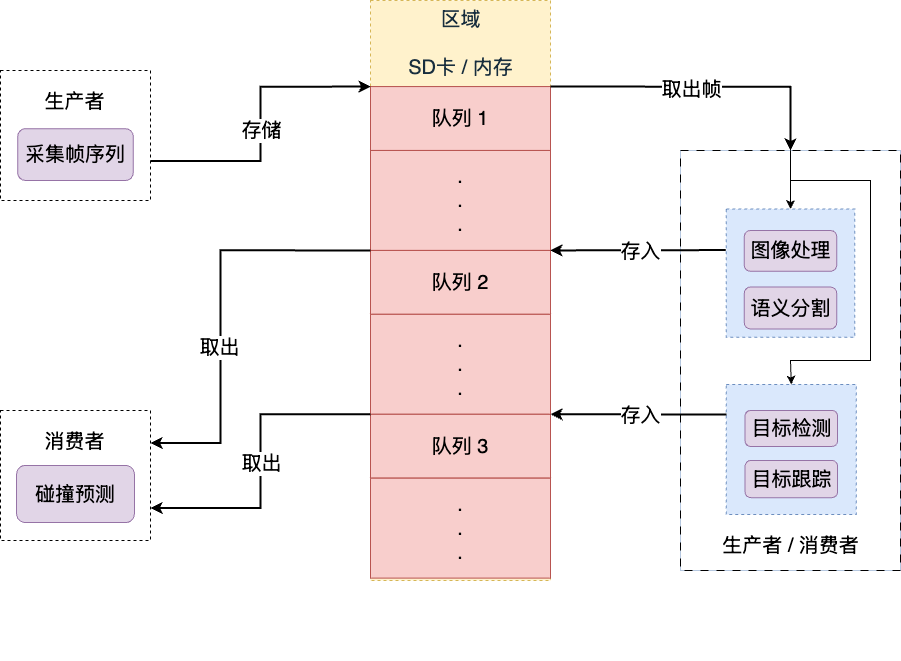
\includegraphics[width=0.8\textwidth]{figures/chapter2/pcm.png}
%     \caption{生产者-消费者模型}
%     \label{fig:pcm}
% \end{figure}

% 为保证多线程环境下的数据安全与有序流转，系统实现了线程安全的队列结构，并通过互斥锁与条件变量等同步机制，防止数据竞争和死锁。例如，当某一处理阶段的队列为空时，消费者线程会自动阻塞等待新数据；当队列已满时，生产者线程则会等待，直到有空余空间。这种机制确保了各处理阶段既能高效并行，又能动态适应系统负载变化，避免了资源浪费和处理瓶颈。

% 此外，通过多种帧缓存模式（如SD卡、RAM、混合模式），根据实际硬件资源动态切换，能够进一步提升了数据流的灵活性和鲁棒性。通过合理设计队列长度和线程数量，系统能够在高负载场景下保持稳定运行，实现了高效、实时的图像处理与碰撞风险评估。


% --------------------------------------------------------------------------------------------------------------------------------------------------------------------------------------------------------------------------------------------------

\newpage
\section{相关理论基础}
\renewcommand{\thefigure}{\thesection.\arabic{figure}}
\renewcommand{\thetable}{\thesection.\arabic{table}}
\renewcommand{\figurename}{图}
\setcounter{figure}{0} % 重置图表计数器
\setcounter{equation}{0} % 重置公式计数器

\subsection{图像处理基础}

作为辅助驾驶感知系统的前端预处理模块，图像处理技术在从原始传感器数据中提取有效信息方面发挥着关键作用。本节介绍的去噪、形态学操作等基础技术构成了环境感知的底层技术基础，其处理质量直接影响后续深度学习模型的性能上限。特别是在复杂交通场景中，路面反光、雨雾干扰等噪声的有效抑制能力，决定了车道线识别、障碍物检测等高级任务的可靠性。

\subsubsection{传统图像增强技术}


数字图像在采集和传输过程中容易受到设备固有噪声、环境干扰等因素的影响，常见的噪声类型包括高斯噪声、椒盐噪声和泊松噪声等。去噪算法的核心在于平衡噪声抑制与图像细节保留，主要方法包括：

\begin{parlist}
\item 中值滤波

中值滤波（Medium Filter）是一种非线性滤波方法，通过滑动窗口内像素值的中位数替代中心像素。其优势在于有效抑制脉冲噪声的同时保持边缘清晰度，计算复杂度为$O(n^2)$，适用于中低分辨率图像处理。数学表达如式\eqref{eq:medium_filter}：

\begin{equation}
\label{eq:medium_filter}
M(x,y) = \text{median}\{ f(i,j)|i \in \lbrack x - k,x + k\rbrack,j \in \lbrack y - k,y + k\rbrack\}
\end{equation}

其中窗口尺寸$k$需根据噪声强度与图像分辨率进行参数调优。在车辆前方障碍物检测中，$3 \times 3$窗口在保持实时性的同时可有效去除雨滴等干扰，如图\ref{fig:medium_filter}所示。

\begin{figure}[H]
\centering
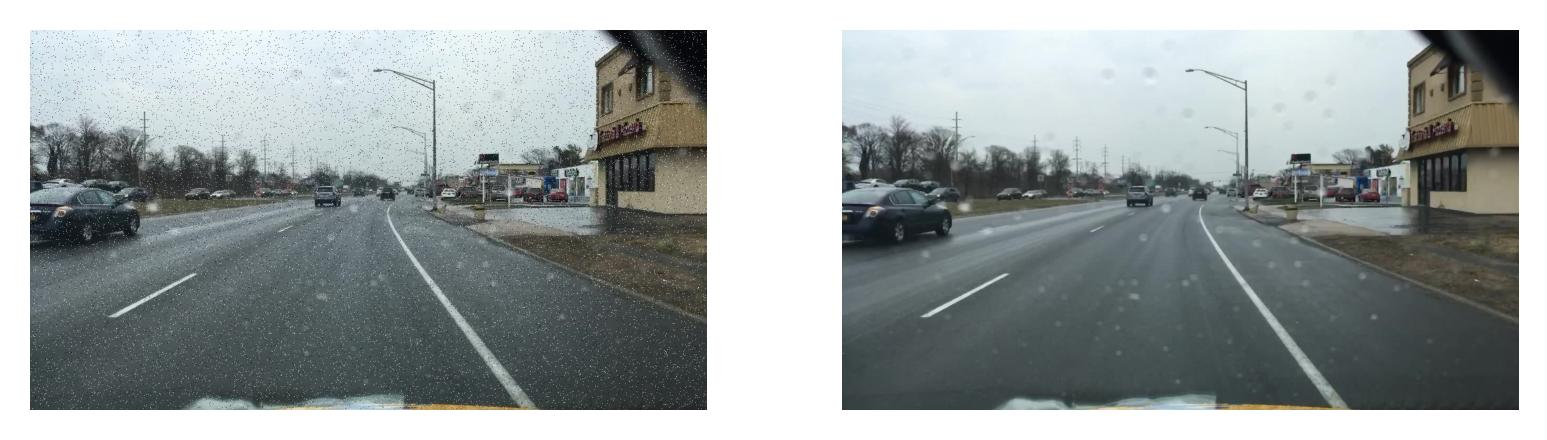
\includegraphics[width=1\textwidth]{figures/chapter2/medium_filtered.jpg}
\begin{center}
(a) 噪声图像 \hspace{4cm} (b) 中值滤波
\end{center}
\caption{中值滤波图}
\label{fig:medium_filter}
\end{figure}

\item 高斯滤波

高斯滤波（Gaussian Filter）是一种线性平滑方法，采用高斯核函数进行加权平均，二维高斯函数如式\eqref{eq:guass_kernel}，特别适合处理图像中符合正态分布的噪声。
\begin{equation}
\label{eq:guass_kernel}
G(x,y) = \frac{1}{2\pi\sigma^2}e^{-\frac{x^2+y^2}{2\sigma^2}}
\end{equation}

标准差$\sigma$决定了平滑强度，较大的$\sigma$可能造成对边缘信息的模糊，而较小的$\sigma$对噪声的抑制不稳定，通过测试，在夜间驾驶场景中，$\sigma=1.8$可有效平衡噪声抑制与边缘保留，如图\ref{fig:gauss_filtered}。
\begin{figure}[H]
\centering
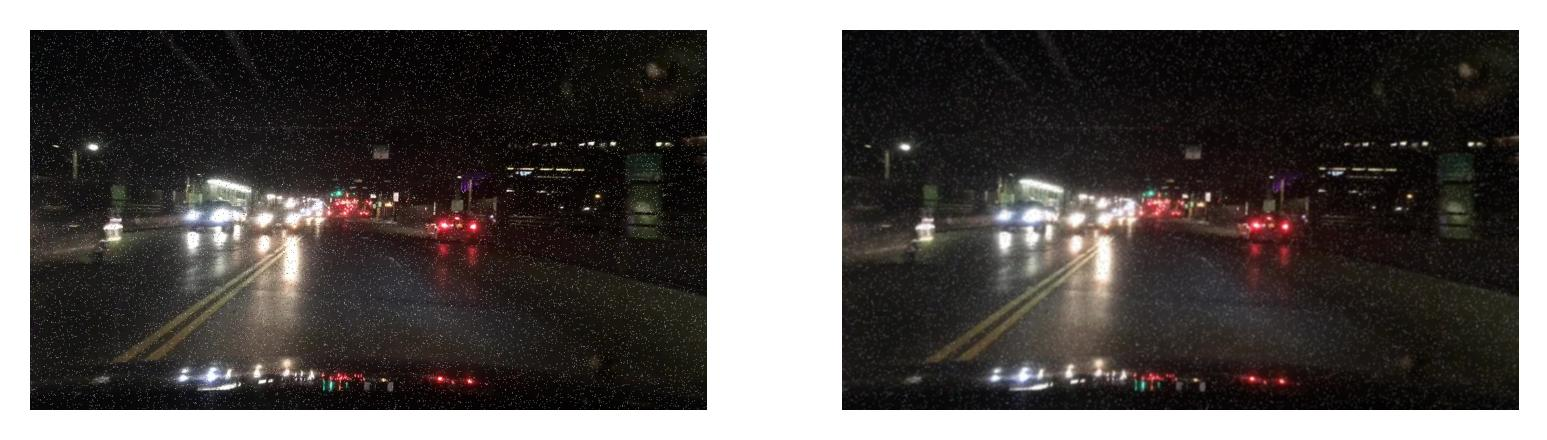
\includegraphics[width=1\textwidth]{figures/chapter2/gauss_filtered.jpg}
\begin{center}
(a) 噪声图像 \hspace{3cm} (b) 高斯滤波
\end{center}
\caption{高斯滤波图}
\label{fig:gauss_filtered}
\end{figure}

\item 双边滤波

双边滤波（Bilateral Filter）结合空间域和像素值域的非线性滤波方法，如式\eqref{eq:bilateral_filter}能够在平滑图像的同时保持边缘信息，与高斯滤波不同，双边滤波的权重依赖于图像本身内容，能够有效应对传统高斯滤波中的边缘丢失问题。

\begin{equation}
\label{eq:bilateral_filter}
BF[I]_p = \frac{1}{W_p}\sum_{q \in S}G_{\sigma_s}(||p-q||)G_{\sigma_r}(|I_p-I_q|)I_q
\end{equation}

其中，$G_{\sigma_s}$为空间核，$G_{\sigma_r}$为值域核，通过该滤波处理，边缘信息能够有效保留。

\item 各向异性扩散滤波

各向异性扩散滤波（Anisotropic Diffusion Filtering）是基于偏微分方程的自适应滤波方法，能够根据局部梯度调整平滑强度，其核心是时变偏微分方程如式\eqref{eq:adf}，通过非跨越式的边缘扩散，自适应调节局部结构，多次迭代可以获得图像多尺度特征，从而适应非均匀光照环境的图像。

\begin{equation}
\label{eq:adf}
\frac{\partial I}{\partial t} = \text{div}(c(|\nabla I|)\nabla I)
\end{equation}

其中$c(\cdot)$为扩散系数，在边缘处减小扩散以保持结构特征，效果如图\ref{fig:ani_diffusion}所示。
\begin{figure}[H]
\centering
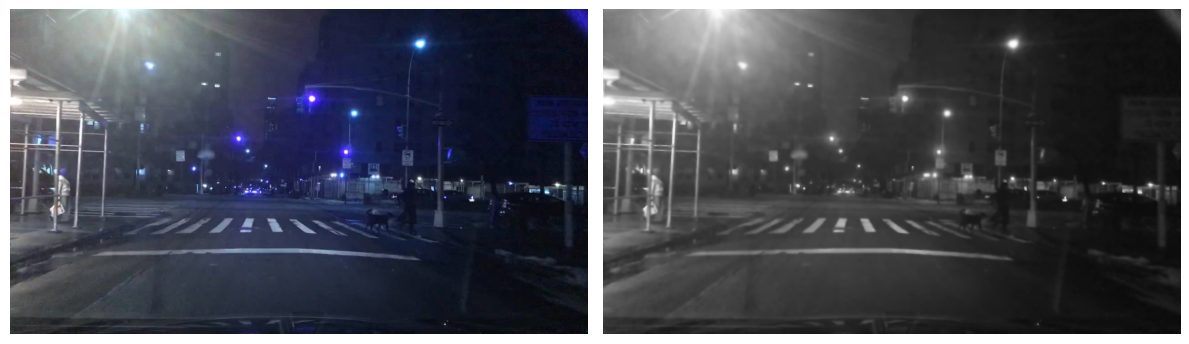
\includegraphics[width=1\textwidth]{figures/chapter2/adf.png}
\begin{center}
(a) 噪声图像 \hspace{3cm} (b) 各向异性扩散滤波
\end{center}
\caption{各向异性扩散滤波图}
\label{fig:ani_diffusion}
\end{figure}

\end{parlist}

在实际车载系统开发中，需根据传感器特性和环境条件选择适配的滤波策略，本文采用的CMOS相机受限于传感器特性易产生椒盐噪声，采用中值滤波预处理；而在低光照条件下，高斯滤波结合亮度自适应阈值可提升夜间视觉效果；对于需要实时处理的场景，可采用积分图技术加速均值滤波，将复杂度降至$O(1)$；对于道路常见的光照不均匀场景，采用各向异性扩散滤波获取更优的特征。

\subsubsection{形态学运算}


形态学处理通过结构化元素操作改变目标区域的拓扑结构，在车道标记和障碍物分割中具有重要应用，其能够连接断裂的车道线、填补路面裂缝反光等

\begin{parlist}
\item 腐蚀运算

\begin{equation}
(A \ominus B)(i,j) = \min_{(x,y) \in B}\{ A(i + x,j + y)\}
\end{equation}

可消除细小噪点但导致目标收缩，在车道线检测中用于分离粘连标记和过滤小面积干扰物。使用$3 \times 3$方形结构元素可去除大部分的环境噪点。

\item 膨胀运算

\begin{equation}
(A \oplus B)(i,j) = \max_{(x,y) \in B}\{ A(i + x,j + y)\}
\end{equation}

膨胀处理能够有效填补目标区域空洞，增强障碍物轮廓连续性，线状结构元素可有效连接断裂的标线段。

\item 开运算与闭运算

\begin{equation}
A \circ B = (A \ominus B) \oplus B
\end{equation}
\begin{equation}
A \bullet B = (A \oplus B) \ominus B
\end{equation}

开运算是对图像先进行腐蚀再进行膨胀，能够有效的消除图像中的小尺寸亮区，从而去除孤立噪声；而闭运算则是对图像先进行膨胀后腐蚀，其特性适用于连接细小缝隙和填补小型凹陷，适用于修补检测盲区。这两种操作都能保持大型物体形状和大小基本不变，实现对图像细小部分的处理。

\item 顶帽变换与底帽变换

\begin{equation}
\text{TopHat}(A) = A - (A \circ B)
\end{equation}
\begin{equation}
\text{BlackHat}(A) = (A \bullet B) - A
\end{equation}

顶帽变换用于提取比背景亮的细小目标，如白色车道线；底帽变换则用于高精度情形下检测黑色物体，如沥青路面上的裂缝。
\end{parlist}


\subsubsection{边缘检测}

边缘提取作为计算机视觉中的基础技术，通过提取图像的轮廓信息，实现特征的有效增强。这一技术广泛应用于计算机视觉、模式识别以及数字影像处理等领域。随着技术发展，边缘检测算法已经从传统的手工设计特征逐步演进至结合深度学习的智能方法。目前，主流的边缘检测算法大致可以分为五类：

\begin{halfparlist}
    \item 基于一阶梯度的检测算法，如Sobel、Prewitt算子，通过计算像素值梯度的幅值与方向识别边界；

    \item 基于二阶导数的检测算法，采用拉普拉斯等二阶差分运算定位边缘区域，如LoG（Laplacian of Gaussian）；

    \item 基于Canny准则的多阶段算法，通过系统化处理实现亚像素级边缘提取；

    \item 基于多尺度分析的高级方法，如DoG（高斯差分）和小波变换，能够捕获不同尺度的边缘特征；

    \item 基于深度学习的端到端方法，如HED、RCF和DexiNed，直接从数据中学习边缘特征表示。
\end{halfparlist}


\begin{parlist}

\item Sobel算子

基于一阶导数的梯度算子，使用分离卷积核加速计算：

\begin{equation}
G_x = \begin{bmatrix} -1 & 0 & +1 \\ -2 & 0 & +2 \\ -1 & 0 & +1 \end{bmatrix} * A
\end{equation}
\begin{equation}
G_y = \begin{bmatrix} -1 & -2 & -1 \\ 0 & 0 & 0 \\ +1 & +2 & +1 \end{bmatrix} * A
\end{equation}
\begin{equation}
G = \sqrt{G_x^2 + G_y^2}
\end{equation}


\item 拉普拉斯算子

基于二阶导数的边缘检测方法：

\begin{equation}
\nabla^2 f = \frac{\partial^2 f}{\partial x^2} + \frac{\partial^2 f}{\partial y^2}
\end{equation}

常用卷积核为：

\begin{equation}
\begin{bmatrix} 0 & 1 & 0 \\ 1 & -4 & 1 \\ 0 & 1 & 0 \end{bmatrix} \text{ 或 } \begin{bmatrix} 1 & 1 & 1 \\ 1 & -8 & 1 \\ 1 & 1 & 1 \end{bmatrix}
\end{equation}

对噪声敏感但能检测到闭合轮廓，通常与高斯滤波组合使用（LoG算子）。


\item Canny算子

Canny边缘检测算子（Canny Edge Detector）通过多阶段处理实现对图像中边缘的精确定位，在复杂路况中可保持连续边缘特征。处理流程为：

\begin{circledlist}
\item 高斯滤波去除噪声
\item 使用Sobel算子计算梯度幅值和方向
\item 非极大值抑制细化边缘
\item 双阈值法确定边缘连接性
\end{circledlist}

\item 多尺度DoG边缘检测

高斯差分（DoG）算子通过计算不同尺度高斯滤波的差值检测边缘，其数学表达式为：

\begin{equation}
DoG(x,y,\sigma_1,\sigma_2) = G(x,y,\sigma_1) - G(x,y,\sigma_2)
\end{equation}

该方法采用多组$\sigma$值（如$(1.0,2.0)$、$(2.0,4.0)$和$(3.0,6.0)$），能够同时捕获不同宽度和清晰度的边缘。小尺度的高斯差分保留细节信息，适合检测清晰的近距离边缘；中等尺度平衡细节与噪声抑制；大尺度则适用于模糊或远处边缘。多尺度融合策略利用不同尺度信息的互补性，显著提升检测完整性。

\item 基于深度学习的边缘检测

深度学习方法通过卷积神经网络实现端到端的边缘检测，代表算法包括：

\begin{circledlist}
\item HED (Holistically-Nested Edge Detection)：利用全卷积网络和深度监督机制，同时结合浅层特征和深层语义信息
\item RCF (Richer Convolutional Features)：整合多层卷积特征，提升边缘检测的精度和语义理解能力
\item DexiNed (Dense Extreme Inception Network)：通过创新的网络结构实现无需预训练的高精度边缘检测
\end{circledlist}

深度学习方法的优势在于能够从数据中自动学习边缘特征表示，区分有语义意义的边缘与无意义的纹理，在复杂场景中表现出优越性能。

\item 混合架构方法

结合传统边缘检测与深度学习的混合架构，形成"白盒+黑盒"的智能系统：

\begin{equation}
E_{final} = \alpha \cdot E_{traditional} + (1-\alpha) \cdot E_{deep}
\end{equation}

其中$\alpha$为自适应权重系数。这种方法融合了传统算法的可解释性和深度学习的高精度特性，通过互补优势提升系统在复杂环境下的鲁棒性。在实际应用中，传统边缘检测方法提供几何约束，深度学习方法提供语义理解，通过熵阈值等机制动态选择最可靠的结果。
\end{parlist}


\subsubsection{拟合车道线}
\begin{parlist}
\item 霍夫变换

霍夫变换（Hough Transform）是用于检测参数化几何形状（如直线、圆、椭圆等）的经典特征提取技术，其核心是将笛卡尔坐标系中的点映射到参数空间，通过累加统计找出最可能的几何形状。

在直线检测中，霍夫变换利用直线的参数表示法。通常，一条直线可以用极坐标形式表示，而笛卡尔空间中位于同一直线上的点，在霍夫参数空间($\rho$-$\theta$平面)中会交于一点。通过在参数空间中构建累加矩阵（accumulator），统计每个参数组合的投票数，从而可以找出最有可能的直线参数。

\begin{equation}
\rho = x\cos\theta + y\sin\theta
\end{equation}

\item 多项式曲线拟合

在获取霍夫变换检测边缘图中的直线段后，对检测到的线段进行分类和过滤，收集分类后的端点作为拟合数据，再应用多项式拟合获得平滑的车道线，利用了霍夫变换在直线检测中的鲁棒性，同时结合复杂曲线的建模能力，可以有效应对复杂车道线情形。
\begin{equation}
y = a_0 + a_1x + a_2x^2 + a_3x^3
\end{equation}

$3$次多项式模型可有效描述弯道曲率，为车道偏离预警提供数学基础如图\ref{fig:polynomial_fit}所示。
\begin{figure}[H]
\centering
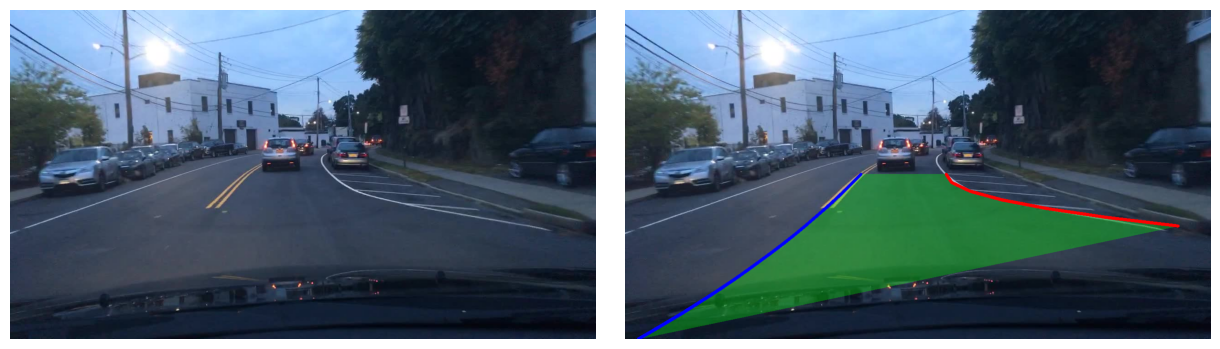
\includegraphics[width=1\textwidth]{figures/chapter2/polynomial_fit.png}
\begin{center}
(a) 原始图像 \hspace{3cm} (b) 多项式拟合
\end{center}
\caption{多项式拟合车道线}
\label{fig:polynomial_fit}
\end{figure}

\end{parlist}


\subsection{语义分割技术}

作为环境感知的核心输出，语义分割质量直接决定路径规划的安全性边界。传统图像处理方法虽能有效提取几何特征，但在复杂场景理解方面存在天然局限。随着智能驾驶系统对环境感知精度和鲁棒性需求的提升，基于深度学习的语义分割技术凭借其强大的特征提取和场景理解能力，逐渐成为道路环境感知的核心技术。

语义分割技术通过为图像中的每个像素分配类别标签，实现了从像素级别对场景的精确理解。这种精细化的场景解析使自动驾驶系统能够准确区分道路、车道线、行人、车辆等关键元素，为后续的路径规划和决策提供可靠的输入。与传统方法相比，深度学习语义分割能够适应各种复杂场景，如光照变化、天气条件恶劣、道路标记模糊等，显著提升了系统的环境适应能力。

在实际部署中，需要在分割精度与计算效率间取得平衡。传统的语义分割网络如FCN、U-Net、DeepLab等虽然在分割精度上表现优异，但计算开销较大，难以满足车载系统的实时性要求。针对这一挑战，轻量化分割网络应运而生，其中Fast-SCNN作为一种专为实时应用设计的轻量级分割网络\cite{poudel2019fast}，在保证分割质量的同时显著降低了计算复杂度，特别适合于资源受限的车载环境。

\subsubsection{FastSCNN}

FastSCNN (Fast Semantic Conditioning Neural Network) 是一种专为边缘设备设计的实时语义分割架构，其核心创新在于提出双路径（two-branch）设计范式，实现高效特征提取与上下文信息捕获的平衡。与传统全卷积网络（FCN）依赖深层次的编码器-解码器结构不同，FastSCNN通过并行的信息处理流显著降低计算量，同时保持强大的分割性能。其数学模型表示为：

\begin{equation}
\label{eq:fastscnn}
\left\{ \begin{array}{ll}
F_{\text{detail}} = \Psi_{\text{HR}}(I) & \text{(高分辨率细节流)} \\
F_{\text{context}} = \Phi_{\text{LR}}(I) & \text{(低分辨率语义流)} \\
F_{\text{output}} = \Gamma(F_{\text{detail}} \otimes F_{\text{context}})
\end{array} \right.
\end{equation}

其中$\otimes$表示特征融合算子，$\Gamma$为解码器函数。该架构设计思想源于观察到语义分割任务中存在的矛盾需求：需要足够大的感受野以获取上下文信息，同时又需要保留高分辨率特征以精确定位边界。FastSCNN通过学习下采样（Learned Downsampling）模块快速降低空间分辨率，在低分辨率分支中提取丰富语义信息，再通过全局特征提取器获取上下文表示，最终与高分辨率特征融合，恢复边缘细节。



\subsubsection{多尺度特征融合策略}

车道线检测面临的主要挑战是细长结构特征的提取和保持，构建了跨尺度特征交互的微分方程模型，通过自适应特征传递路径实现不同分辨率信息的有效融合：

\begin{equation}
\label{eq:routing}
r_{ij} = \frac{exp(s_{ij})}{\sum_{k}^{}\exp(s_{ik})},\quad s_{ij} = \langle W_{q}f_{i},W_{k}f_{j}\rangle
\end{equation}
其中$r_{ij}$表示特征图$i$与特征图$j$之间的路由强度，$W_q$和$W_k$分别为查询和键值变换矩阵，$\langle\cdot,\cdot\rangle$表示内积操作。该机制使网络能够根据输入图像的复杂度自适应地调整信息流，对于简单场景保持高效处理，而对于复杂场景则激活更深层的特征交互。

此外，采用基于类别加权的损失函数，增强模型对安全关键区域的识别能力，这种权重设置反映了道路场景中非道路区域的安全优先级，使模型在训练过程中更关注这些潜在风险区域的准确分割。

\subsubsection{传统方法与深度学习协同机制}

为克服单一方法的局限性，建立了传统计算机视觉方法与深度学习模型相结合的混合式分割框架：

\begin{equation}
\label{eq:hybrid}
\widehat{M} = \underset{深度学习}{\underbrace{\mathcal{N}_{DL}(I)}} \oplus \underset{传统方法}{\underbrace{\mathcal{T(}I)}}
\end{equation}

这种协同机制为系统带来三重优势：首先，传统边缘检测方法提供了可解释的几何约束，对FastSCNN输出进行校正；其次，形态学操作（如闭运算）有效填补了深度学习模型在细节区域可能产生的空洞；最后，通过熵阈值判断，系统能够智能切换至最可靠的处理结果，实现"有理有据"的决策过程。在实际部署中，多项式曲线拟合模块对边缘检测结果进行数学建模。

这种"白盒+黑盒"的混合架构体现了本研究的核心方法论——在数据驱动的智能模型中注入物理可解释性，使其既保有深度学习的抽象能力，又具备传统算法的稳定内核。

\subsection{目标检测及目标跟踪理论}


语义分割为环境提供了像素级的理解，而目标检测则进一步实现了对场景中独立实体的识别与定位。在智能驾驶场景中，准确检测和跟踪道路上的各类移动障碍物是避免碰撞的前提。
现代目标检测技术已由早期的传统特征提取方法（如HOG、SIFT等）发展为基于深度学习的端到端解决方案，大幅提升了检测精度和鲁棒性。

目标跟踪作为智能驾驶感知系统的关键环节，承担着将离散检测结果关联为连续时空轨迹的核心任务。
在复杂交通场景中，遮挡、相似外观目标、光照变化等因素使得稳定跟踪面临巨大挑战。本研究选择DeepSORT作为基础框架，通过多项创新设计增强其在车载环境中的鲁棒性。

作为感知系统的纵深防线，目标检测与跟踪系统不仅需要精准识别各类交通实体，还需要预测它们的运动状态与意图。
这种时空维度的理解为后续的碰撞风险评估提供了必要基础。
本节将首先介绍YOLOv5目标检测算法的理论框架，然后详细阐述DeepSORT多目标跟踪系统的核心机制，最后探讨针对车载环境的优化策略。

\subsubsection{目标检测算法YOLOv5}

作为实时目标检测领域的里程碑式算法，YOLO (You Only Look Once) 系列通过单阶段端到端的检测范式重新定义了计算机视觉任务的效率标准。
YOLOv5作为该系列的重要迭代，在保持实时性的同时显著提升了检测精度，特别适合计算资源受限的车载环境。
\begin{parlist}
\item 理论基础与架构演进

YOLOv5的核心理论基础建立在单阶段检测器的创新模型上，其通过将目标检测问题转化为回归问题，实现了端到端的推理过程。
与两阶段检测器（如R-CNN系列）不同，YOLOv5直接从输入图像预测边界框坐标和类别概率，避免了候选区域生成和二次分类的计算开销。其理论框架可表述为：

\begin{equation}
f(I) \mapsto \{(b_i, c_i, p_i) | i \in [1, N]\}
\end{equation}

其中$I$为输入图像，$b_i$为第$i$个预测框的坐标参数$[x, y, w, h]$，$c_i$为类别，$p_i$为置信度。

YOLOv5架构引入多项关键创新，包括CSP结构、PANet特征融合、Focus模块和自适应锚框计算。其中，CSP模块通过跨阶段局部连接优化梯度流动，可表示为：

\begin{equation}
Y = Concat(Conv_{1 \times 1}(X_1), BottleNeck(X_2))
\end{equation}

\item 多尺度检测机制

YOLOv5针对交通场景中远近目标共存的特点，设计了三级检测头结构，实现全尺度目标的有效捕获：

\begin{equation}
P = \{P_l, P_m, P_s\}
\end{equation}

其中$P_l$、$P_m$、$P_s$分别对应大、中、小三种尺度的特征图，分别负责检测近、中、远距离目标。通过特征金字塔网络（FPN）和路径聚合网络（PAN）的双向连接，实现了自顶向下和自底向上的信息流动：

\begin{equation}
\begin{aligned}
P_l &= Conv(Backbone_{stage5}) \\
P_m &= Conv(Upsample(P_l) \oplus Backbone_{stage4}) \\
P_s &= Conv(Upsample(P_m) \oplus Backbone_{stage3})
\end{aligned}
\end{equation}

这种双向特征融合机制显著增强了模型对不同尺度目标的检测能力，在车载环境中能够同时精确识别远处的行人和近处的车辆。

\item 模型系列与轻量化设计

YOLOv5提供了不同复杂度的模型变体（YOLOv5n/s/m/l/x），但无论哪种模型，其Backbone，Neck，Output都是一致的，区别在于模型深度和宽度设置。如图\ref{fig:yolov5-comparison}所示。
\begin{figure}[H]
\centering
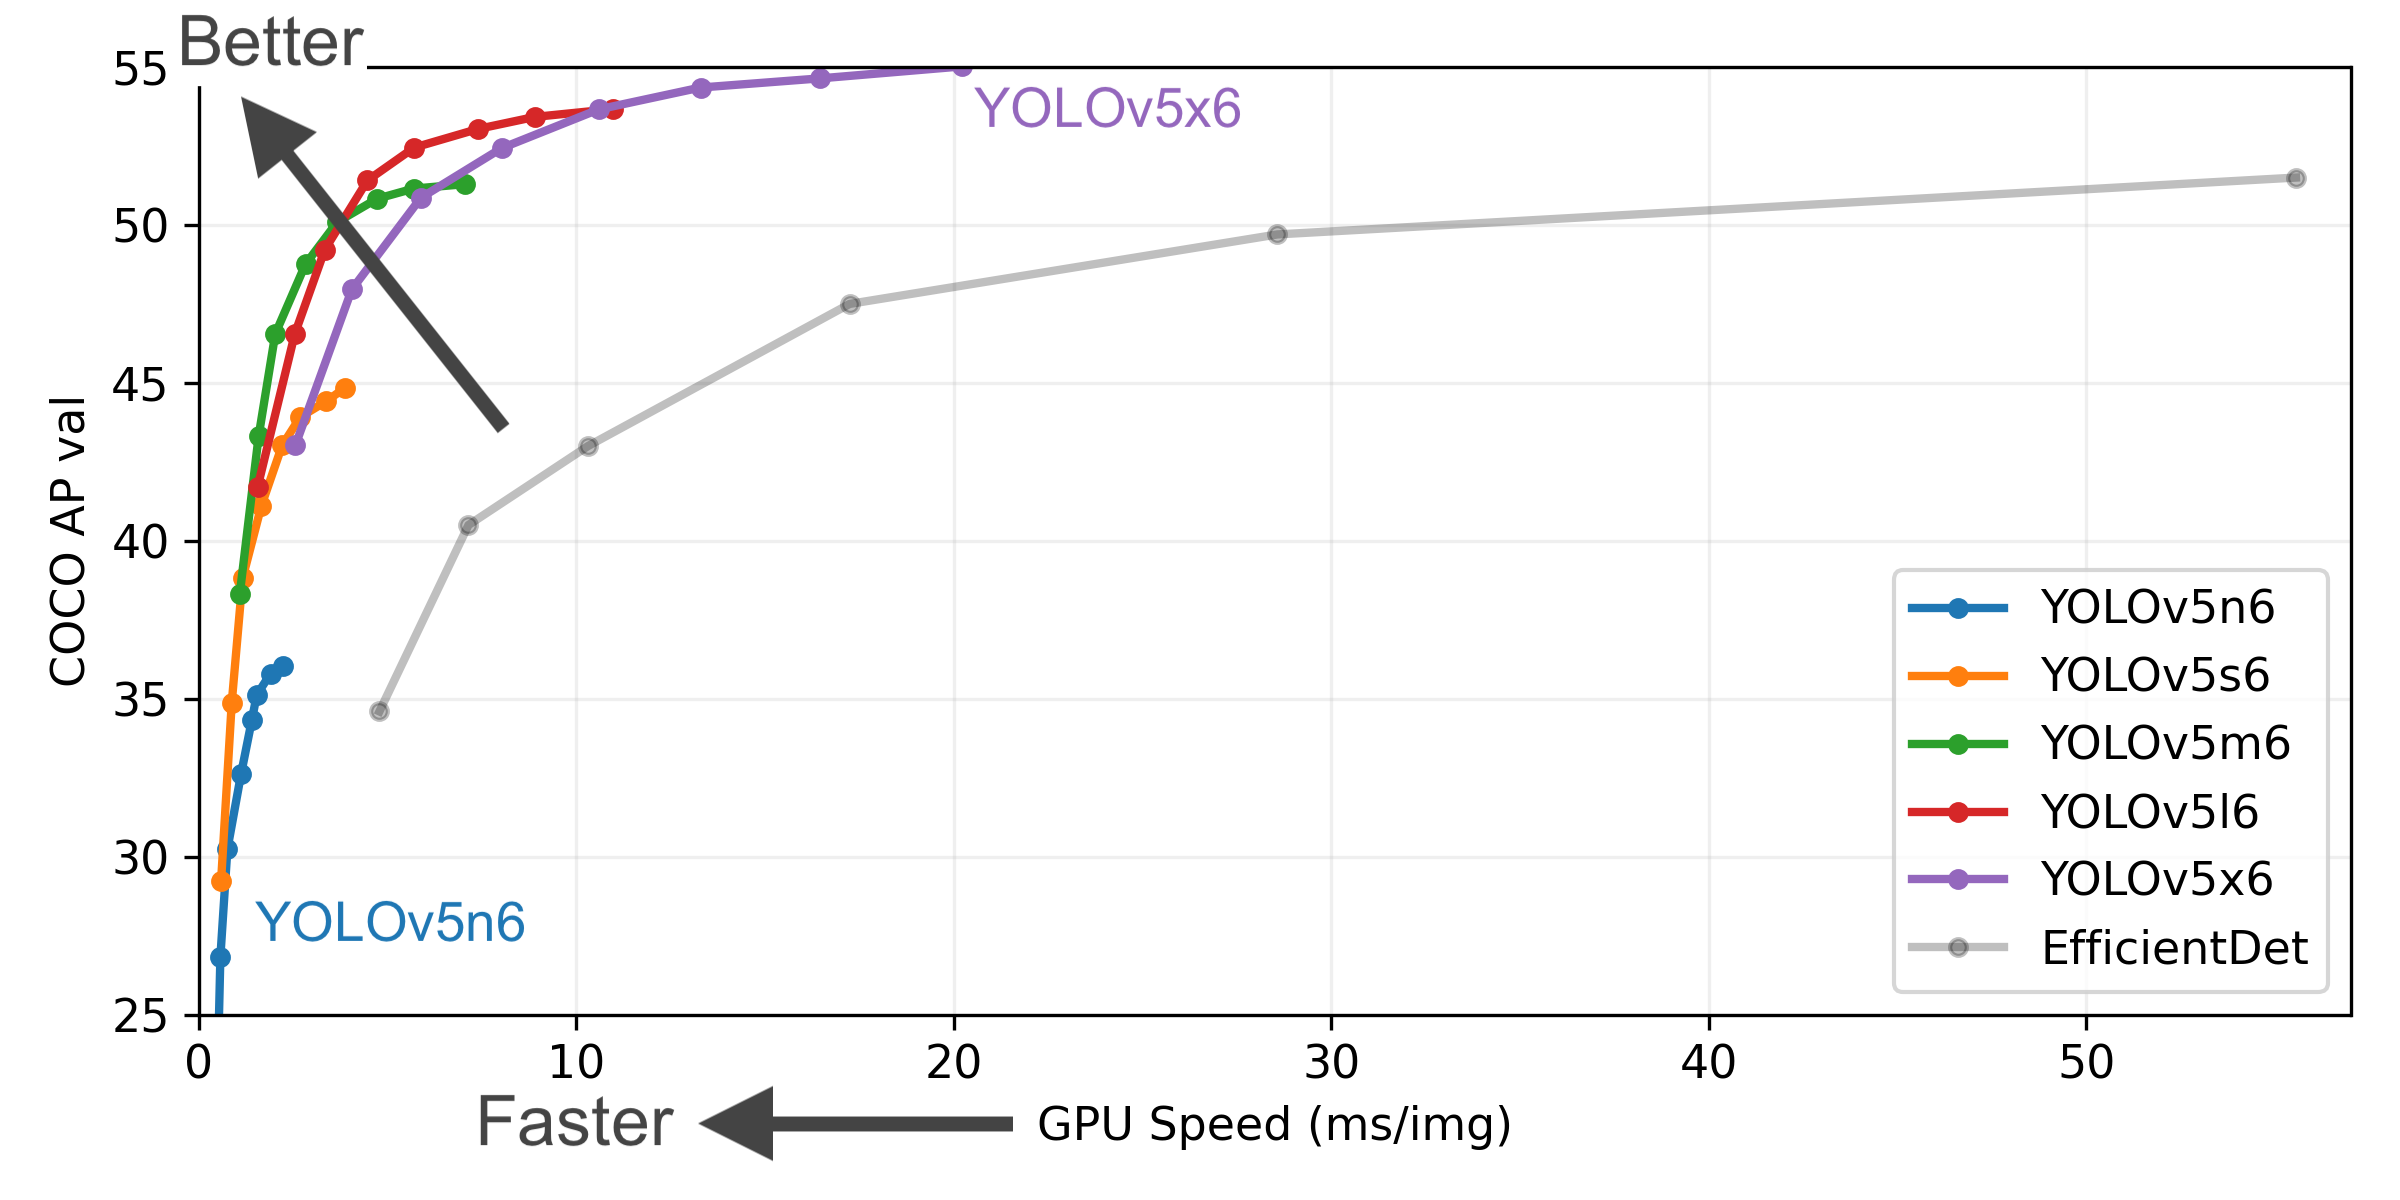
\includegraphics[width=1\textwidth]{figures/chapter2/yolov5.png}
\caption{YOLOv5模型在COCO数据集测试结果}
\label{fig:yolov5-comparison}
\end{figure}

各个尺度的预训练参数如表\ref{tab:yolov5-params}所示。
\begin{table}[H]
\centering
\caption{YOLOv5模型系列参数对比}
\label{tab:yolov5-params}
\begin{tabular}{lccccc}
\hline
\textbf{模型} & \textbf{参数量} & \textbf{计算量(GFLOPs)} & \textbf{mAP@0.5} & \textbf{推理速度(FPS)} \\
\hline
YOLOv5n & 1.9M & 4.5 & 45.7\% & 260 \\
YOLOv5s & 7.2M & 16.5 & 56.8\% & 220 \\
YOLOv5m & 21.2M & 48.0 & 64.1\% & 150 \\
YOLOv5l & 46.5M & 109.1 & 67.3\% & 95 \\
YOLOv5x & 86.7M & 205.7 & 68.9\% & 65 \\
\hline
\end{tabular}
\end{table}

其中YOLOv5n（nano）专为边缘计算设备设计，通过减少网络深度和宽度显著降低了计算开销。其轻量化策略包括深度与宽度动态调整、Group Convolution、SiLU激活函数优化以及知识蒸馏与量化技术。
本研究采用YOLOv5n为基础，结合车载场景的特点进行了针对性优化，包括类别优先级差异化、注意力增强模块和多帧时序融合等技术。

另外使用了YOLOv5s模型作为蒸馏的教师模型，对YOLOv5n低参数模型进行优化，有效提高了对车载环境下障碍物的检测能力，同时降低了部署于边缘的资源消耗。
\item 损失函数优化

作为检测性能的关键驱动因素，采用EIoU（Efficient Intersection over Union）损失函数改进边界框回归精度。针对传统IoU度量对边界框尺度不敏感的问题，EIoU通过引入中心点距离惩罚项和宽高差异补偿机制，构建了更符合目标检测任务特性的回归目标：

\begin{equation}
\mathcal{L}_{EIoU} = 1 - IoU + \frac{\rho^2(b_{pred},b_{gt})}{c^2} + \frac{\rho^2(w_{pred},w_{gt}) + \rho^2(h_{pred},h_{gt})}{c_w^2 + c_h^2}
\end{equation}

其中$\rho(\cdot)$表示欧氏距离，$c$为最小包围框对角线长度，$c_w$、$c_h$为包围框宽高。与CIoU相比，EIoU解耦了宽高方向的梯度更新，使网络能够更精确地学习目标几何特征。
\end{parlist}


\subsubsection{目标跟踪算法DeepSORT}

\begin{parlist}


\item 目标跟踪算法发展

目标跟踪是计算机视觉领域的核心研究方向，其目的是在连续视频帧序列中确定目标物体的运动轨迹。随着智能驾驶、视频监控等应用场景的快速发展，多目标跟踪技术经历了从传统方法到深度学习方法的演进过程。

早期的目标跟踪主要聚焦于单目标场景，采用基于高斯模型的背景差分、基于边缘和颜色的形状描述符等方法。然而，这些传统方法在复杂环境下表现不佳，特别是在目标遮挡、快速运动、光照变化等挑战性场景中往往失效。多目标跟踪技术的出现，旨在同时追踪多个运动目标并维持其身份一致性，但初期的多目标跟踪算法仍面临精度与实时性的平衡问题。


\item{DeepSORT算法架构与工作原理}

DeepSORT（Deep Simple Online and Realtime Tracking）算法是由Wojke等人在2017年提出的多目标跟踪算法\cite{wojke2017simple}，它在原有SORT算法的基础上引入深度学习特征提取模块，构建了一个高效且鲁棒的跟踪系统。该算法采用"检测-跟踪"范式，具有模块化架构，主要包含以下四个核心组件：

\begin{circledlist}
    \item 检测关联模块

    DeepSORT首先利用目标检测器（如YOLO、Faster R-CNN等）获取每帧图像中的目标检测框，然后将当前帧的检测结果与现有轨迹进行关联。关联过程采用级联匹配策略，通过计算检测框与轨迹之间的马氏距离（spatial distance）和外观特征距离（appearance feature distance）的加权组合，构建代价矩阵，并使用匈牙利算法求解最优匹配问题。

    \item 卡尔曼滤波模块

    对每个跟踪目标，DeepSORT维护一个卡尔曼滤波器，用于估计目标的运动状态（包括位置、速度等）。卡尔曼滤波器包含预测和更新两个阶段：预测阶段根据上一时刻的状态推测当前状态；更新阶段根据实际测量值修正状态估计。这一机制使算法能够有效处理目标短时遮挡和检测失败的情况。

    \item 外观特征提取模块

    DeepSORT的核心创新在于引入了深度学习特征提取网络，该网络通常采用具有度量学习能力的卷积神经网络，如在行人重识别数据集上预训练的Siamese网络。对每个检测框区域，特征提取网络生成固定维度的特征向量，用于计算目标间的外观相似度，这极大提高了算法在复杂场景中区分相似目标的能力。

    \item 轨迹管理模块

    负责轨迹的初始化、维护和终止。当检测到新目标且无法与现有轨迹关联时，算法会初始化一个新轨迹；连续多帧未能关联到检测结果的轨迹会被标记为丢失，并在达到预设阈值后终止。轨迹管理机制还包含轨迹平滑和抑制短期误检测的策略，提高了算法的稳定性。
\end{circledlist}

DeepSORT算法相比传统方法具有以下显著优势：鲁棒性增强，通过融合深度学习特征与运动信息，能够在目标遮挡、外观相似等复杂场景下保持稳定的跟踪表现；身份保持能力，深度特征的引入大幅减少了ID切换（identity switch）现象；实时处理能力，在主流硬件上可达到实时或近实时性能；以及模块化设计，便于针对特定应用场景进行定制化改进。
在实际应用中，DeepSORT已广泛应用于智能交通系统、视频监控、行人分析及智能驾驶等领域。特别在智能驾驶场景中，DeepSORT能有效跟踪周围车辆、行人等交通参与者，为路径规划和碰撞预警提供关键信息支持。

\end{parlist}





% --------------------------------------------------------------------------------------------------------------------------------------------------------------------------------------------------------------------------------------------------
\newpage
\renewcommand{\thefigure}{\thesection.\arabic{figure}}
\renewcommand{\thetable}{\thesection.\arabic{table}}
\renewcommand{\figurename}{图}
\setcounter{figure}{0} % 重置图表计数器
\setcounter{equation}{0} % 重置公式计数器

\section{车道规划}
\subsection{车道线提取}

对于车道线的提取以及车辆预行区域的规划，是整个系统的核心环节。其结果直接影响碰撞预测的准确性。因此，相关处理的精度和鲁棒性至关重要。
本研究针对车道线检测任务构建了多阶段处理框架，如算法\ref{alg:lane_detection}所示。该框架结合了传统图像处理与现代计算机视觉技术，显著提高了车道线检测的准确性与鲁棒性。


\begin{algorithm}[H]
\caption{车道线检测算法}
\label{alg:lane_detection}
\begin{algorithmic}[1]
\REQUIRE 道路场景图像 $Input Image$
\ENSURE 车道线参数 $P_{left}$, $P_{right}$

\STATE 颜色分割：提取图像中的黄色和白色区域
\begin{align*}
    M_{color} &= ColorSegmentation(I)
\end{align*}

\STATE 多尺度DoG边缘检测：应用不同尺度的高斯差分
\begin{align*}
    E_{dog} &= \bigcup_{i=1}^{n} DoG(G_{\sigma_{1i}}(M_{color}), G_{\sigma_{2i}}(M_{color}))
\end{align*}

\STATE 边缘增强：通过形态学运算优化边缘
\begin{align*}
    E_{enhanced} &= Morphology(E_{dog})
\end{align*}

\STATE 区域限定：应用ROI掩码
\begin{align*}
    E_{roi} &= E_{enhanced} \cap M_{roi}
\end{align*}

\STATE 直线检测：霍夫变换检测直线段
\begin{align*}
    L_{left}, L_{right} &= HoughLinesP(E_{roi})
\end{align*}

\STATE 车道线拟合：多项式拟合
\begin{align*}
    P_{left} &= PolyFit(L_{left}, 2) \\
    P_{right} &= PolyFit(L_{right}, 2)
\end{align*}

\RETURN $P_{left}$, $P_{right}$
\end{algorithmic}
\end{algorithm}

\noindent\rule{\textwidth}{0.4pt}


\subsubsection{颜色分割}
将RGB图像转换为HSV色彩空间，提取车道线区域（主要是黄色和白色），如图\ref{fig:color_seg}所示。HSV色彩空间对光照变化不敏感，能有效减少背景干扰。与RGB空间相比，HSV空间更有效地分离色相、饱和度和亮度信息，使算法在不同照明条件下保持较高鲁棒性。经过颜色分割后，路面纹理、周围车辆和地面阴影等干扰元素得到显著抑制，为边缘检测提供高质量输入。

\begin{figure}[H]
    \centering
    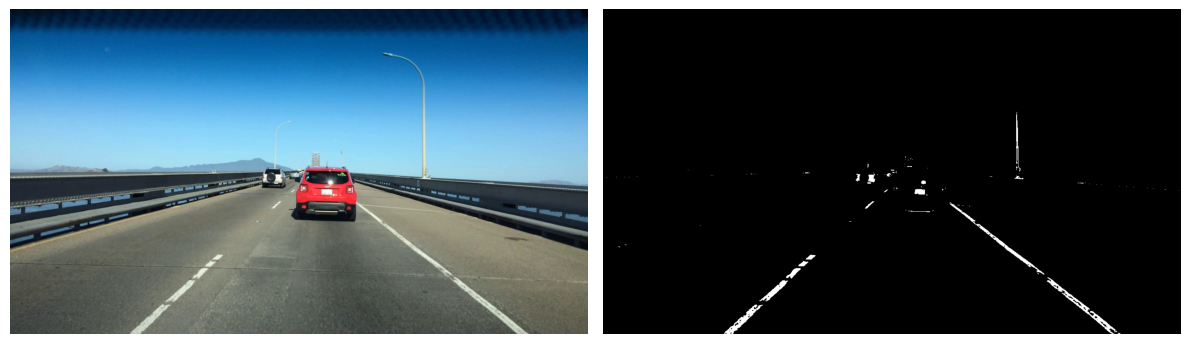
\includegraphics[width=0.8\textwidth]{figures/chapter3/1_color_segmentation.png}
    \begin{center}
    (a) 原始图像 \hspace{3cm} (b) 颜色分割结果
    \end{center}
    \caption{颜色分割处理效果图}
    \label{fig:color_seg}
\end{figure}

\subsubsection{多尺度DoG边缘检测}

如图\ref{fig:dog_edge}所示，高斯差分（DoG）算子通过计算不同尺度高斯滤波的差值检测边缘。采用多组$\sigma$值（$(1.0,2.0)$、$(2.0,4.0)$和$(3.0,6.0)$），捕获不同宽度和清晰度的车道线。小尺度的高斯差分保留细节信息，适合检测近处清晰的车道线；中等尺度平衡细节与噪声抑制；大尺度则应对模糊或磨损的远处车道线。多尺度融合策略利用不同尺度信息的互补性，显著提升检测完整性。

\begin{figure}[H]
    \centering
    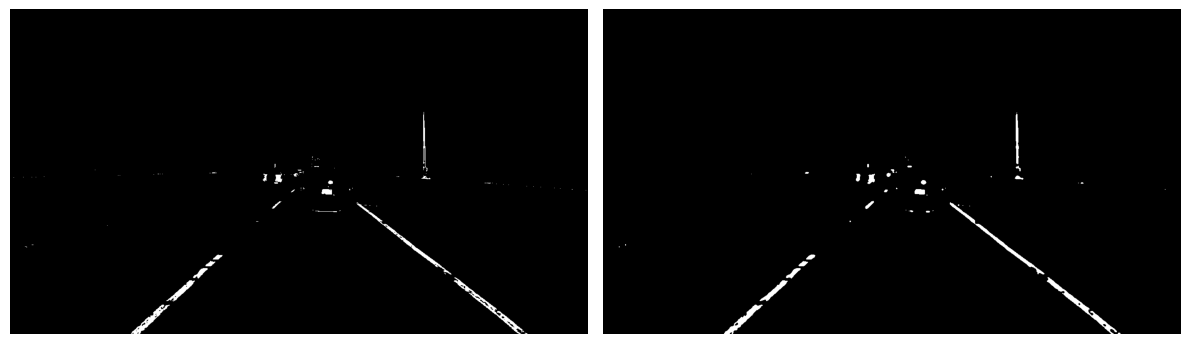
\includegraphics[width=0.8\textwidth]{figures/chapter3/2_dog_edge_detection.png}
    \begin{center}
    (a) 颜色分割结果 \hspace{3cm} (b) DoG边缘检测结果
    \end{center}
    \caption{多尺度DoG边缘检测效果图}
    \label{fig:dog_edge}
\end{figure}

\subsubsection{边缘增强}

通过形态学处理增强边缘连续性，解决车道线断裂或模糊问题，如图\ref{fig:edge_enhance}所示。首先应用顶帽变换突出比周围区域亮的细节结构；随后的闭运算（先膨胀后腐蚀）填充微小间隙，连接相近边缘点；开运算（先腐蚀后膨胀）去除孤立噪点；最后的膨胀操作增强边缘可见度。这一多阶段形态学处理显著提高了车道线的完整性和连贯性，为几何分析奠定基础。

\begin{figure}[H]
    \centering
    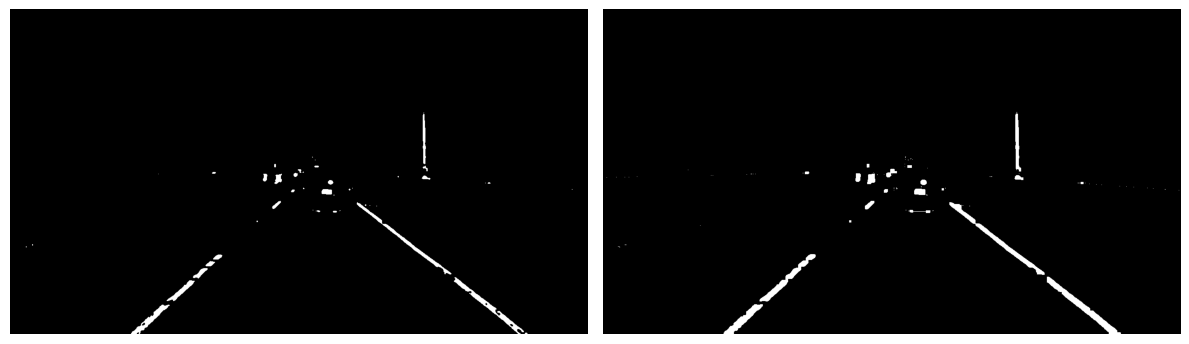
\includegraphics[width=0.8\textwidth]{figures/chapter3/3_edge_enhancement.png}
    \begin{center}
    (a) DoG边缘检测结果 \hspace{3cm} (b) 形态学增强后结果
    \end{center}
    \caption{边缘增强处理效果图}
    \label{fig:edge_enhance}
\end{figure}

\subsubsection{区域限定}

定义梯形ROI（感兴趣区域），如图\ref{fig:roi}所示，仅保留图像下部可能含车道线的区域。梯形上部较窄对应远处汇聚的车道线，下部较宽匹配近处分散的车道线。区域限定不仅降低了计算复杂度，提高算法实时性，还有效排除了图像上部的天空、建筑物和植被等非关键区域。图\ref{fig:roi_mask}展示ROI蒙版应用效果。

\begin{figure}[H]
    \centering
    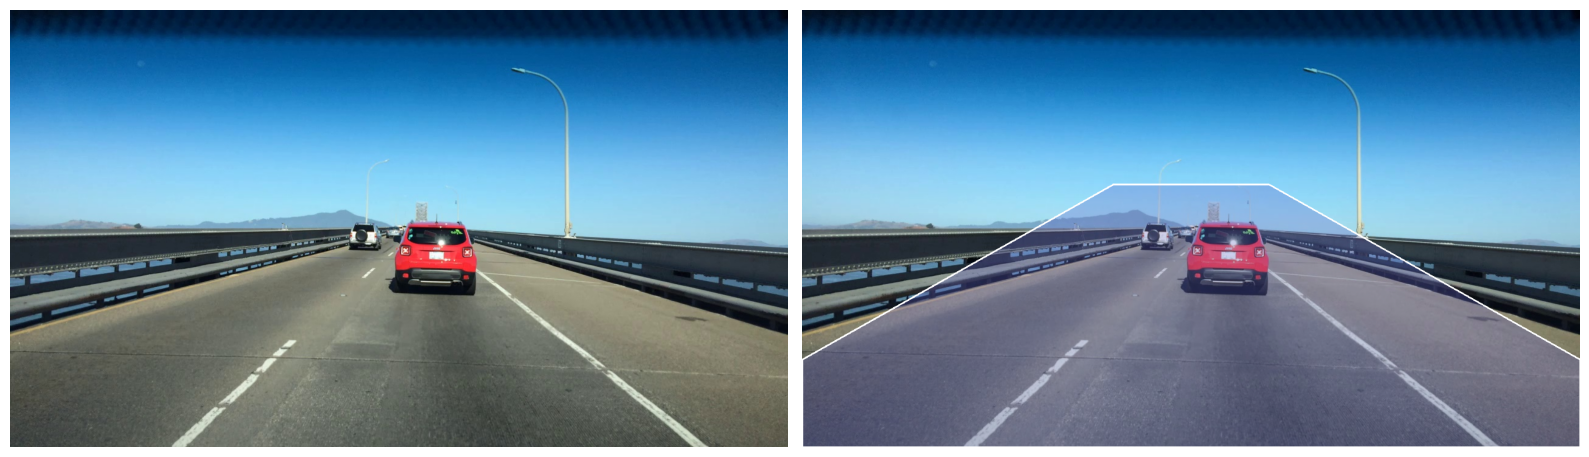
\includegraphics[width=0.8\textwidth]{figures/chapter3/roi_comparison.png}
    \begin{center}
    (a) 原始图像 \hspace{3cm} (b) ROI区域可视化
    \end{center}
    \caption{ROI区域定义图}
    \label{fig:roi}
\end{figure}

\begin{figure}[H]
    \centering
    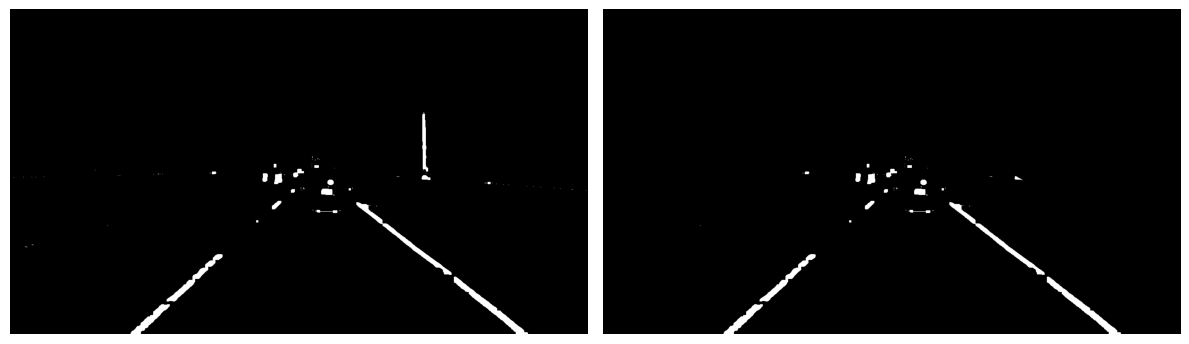
\includegraphics[width=0.8\textwidth]{figures/chapter3/4_roi_masking.png}
    \begin{center}
    (a) 边缘增强结果 \hspace{3cm} (b) ROI掩码应用结果
    \end{center}
    \caption{ROI掩码应用效果图}
    \label{fig:roi_mask}
\end{figure}

\subsubsection{直线检测}

应用概率霍夫变换检测边缘图中的直线段，如图\ref{fig:line_detect}所示。根据斜率将检测到的线段分为左右两组（负斜率为左，正斜率为右），同时过滤接近水平的线段（$|slope| < 0.4$）。概率霍夫变换通过将笛卡尔空间中的点映射到霍夫参数空间，将线段检测转化为峰值查找问题。斜率过滤机制有效去除横向车道标记、路面裂缝等无关线段，提高后续拟合精度。

\begin{figure}[H]
    \centering
    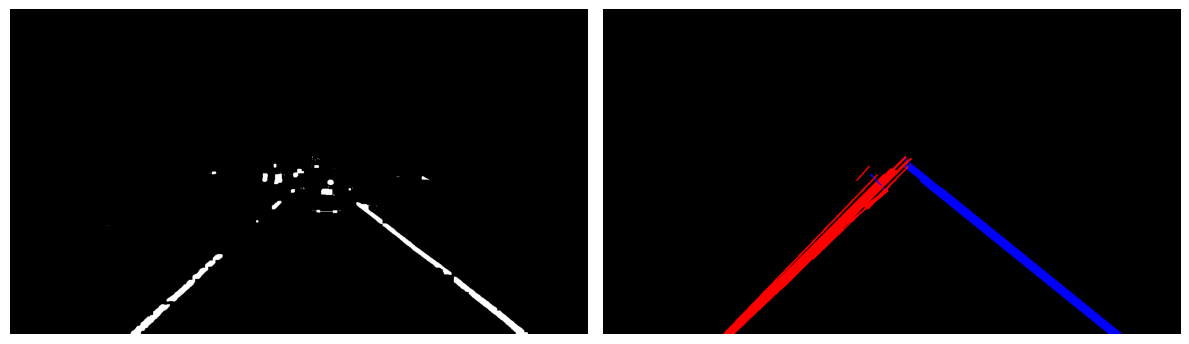
\includegraphics[width=0.8\textwidth]{figures/chapter3/5_line_detection.png}
    \begin{center}
    (a) ROI掩码处理结果 \hspace{3cm} (b) 直线检测结果
    \end{center}
    \caption{霍夫变换直线检测效果图}
    \label{fig:line_detect}
\end{figure}

\subsubsection{车道线拟合}
如图\ref{fig:lane_fit}所示，对分类后的线段点集应用二次多项式拟合，获得平滑连续的车道线表示。二次多项式形式为$x = ay^2 + by + c$，以$y$为自变量、$x$为因变量。拟合过程采用最小二乘法，通过最小化拟合曲线与实际点集间的平方误差和，得到最优参数。二次多项式模型适合道路曲率变化平缓的特点，避免高阶多项式的过拟合风险。最终检测结果如图\ref{fig:final_result}所示。

\begin{figure}[H]
    \centering
    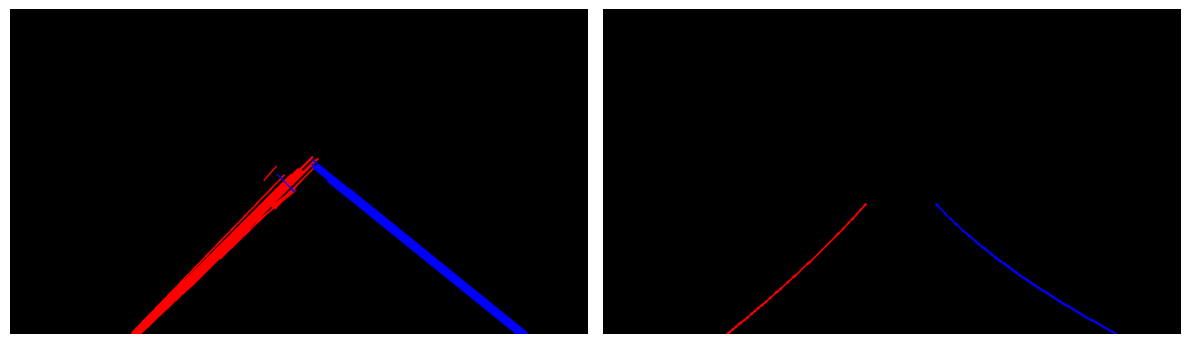
\includegraphics[width=0.8\textwidth]{figures/chapter3/6_lane_fitting.png}
    \begin{center}
    (a) 检测到的直线段 \hspace{3cm} (b) 多项式拟合结果
    \end{center}
    \caption{车道线拟合效果图}
    \label{fig:lane_fit}
\end{figure}

\begin{figure}[H]
    \centering
    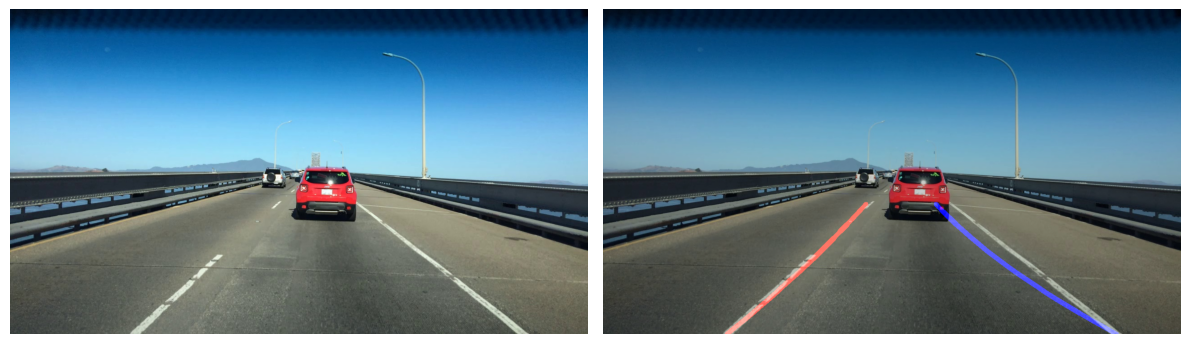
\includegraphics[width=0.8\textwidth]{figures/chapter3/7_final_result.png}
    \begin{center}
    (a) 原始图像 \hspace{3cm} (b) 车道线检测结果
    \end{center}
    \caption{车道线检测结果}
    \label{fig:final_result}
\end{figure}


提取车道线后，获得了较为准确的真实车道信息，为后续的安全预行区域确定提供了基础。

\subsection{FastSCNN推理}
传统图像处理方法在车道线检测中虽有一定效果，但易受图像噪点、曝光异常、光照变化和复杂路面纹理等因素影响，尤其在恶劣天气条件下表现不佳。为提高系统在多样环境下的鲁棒性，本研究引入深度学习模型FastSCNN，进行道路场景语义分割，实现对行驶区域的精确识别。FastSCNN作为一种轻量级实时语义分割网络，平衡了精度与推理速度，特别适合车载嵌入式系统部署需求。

\subsubsection{数据集选取}
本研究采用KITTI道路数据集作为模型训练和评估的基础。KITTI是自动驾驶领域的标准数据集之一，包含多种驾驶场景下的高质量图像和精确标注，涵盖城市、乡村和高速公路等不同道路环境。该数据集提供约290张训练图像和290张测试图像，分辨率为1242×375像素，每张图像都有对应的二值掩码标注，清晰区分可行驶与非可行驶区域。

数据集多样性主要体现在三个方面：不同光照条件（从明亮日光到阴影交错的复杂场景）；多样路面类型（包括沥青路面、混凝土路面和部分损坏路面）；以及复杂交通场景（含车辆、行人、交通标志和各种道路标记等干扰因素）。这种多样性有助于训练出适应性强、泛化能力好的模型。

\subsubsection{预处理}
数据预处理是确保模型训练效果的关键环节。本研究使用KITTI数据集提供的二值掩码作为标注，并设计了专门的数据加载和增强流程。首先，通过自定义KittiRoadDataset类实现高效数据读取与管理，建立图像与掩码间的映射关系。针对训练过程，引入多种数据增强策略以提高模型泛化能力：
\begin{circledlist}
\item 尺寸调整：将图像统一调整至320×800分辨率，符合FastSCNN输入要求，同时保持足够细节信息；
\item 水平翻转：以50\%概率应用，增加训练样本多样性；
\item 亮度和对比度调整：随机变换图像亮度与对比度，模拟不同光照条件；
\item 高斯噪声：添加随机噪点，提高模型抗噪能力；
\item 标准化：应用ImageNet预训练模型的均值和标准差进行标准化，加速收敛。
\end{circledlist}
数据集按8:2比例划分为训练集和验证集，确保模型在训练过程中得到有效评估。这些预处理步骤不仅提高了训练数据质量和多样性，还显著改善了模型的学习效率和泛化能力。

\subsubsection{模型训练}
FastSCNN模型的训练过程经过精心设计，以平衡精度、训练效率和资源消耗。训练采用了多项优化技术提高性能：

在模型架构方面，使用了改进的EnhancedFastSCNN结构，保留原始FastSCNN的学习分支结构，同时优化了特征提取和融合模块，提高细节保留能力。模型针对道路分割任务特化，输出类别设为2（可行驶区域和非可行驶区域）。

损失函数方面，采用加权交叉熵损失，对道路类别赋予更高权重（4:1），有效缓解数据不平衡问题，提高道路区域识别精度。优化器选用AdamW并配合权重衰减（1e-4）控制模型复杂度，防止过拟合。

学习率调度采用OneCycleLR策略，训练初期快速提高学习率至峰值，随后逐渐降低，加速收敛并提高稳定性。训练过程采用混合精度训练和梯度裁剪（阈值1.0）技术，显著减少显存消耗，同时防止梯度爆炸。

训练在多GPU环境下进行，通过DataParallel实现数据并行处理，充分利用硬件资源。批次大小根据可用GPU数量动态调整，平衡训练速度和内存使用。整个过程持续监测验证集性能，保存最佳mIoU模型，防止过拟合。

\subsubsection{模型评估}
FastSCNN模型在KITTI道路数据集验证集上进行了全面评估，主要采用平均交并比（mIoU）作为评价指标，同时分析各类别IoU性能。如图\ref{fig:fastscnn_training}所示，模型训练展现了稳定的收敛趋势。

\begin{figure}[H]
    \centering
    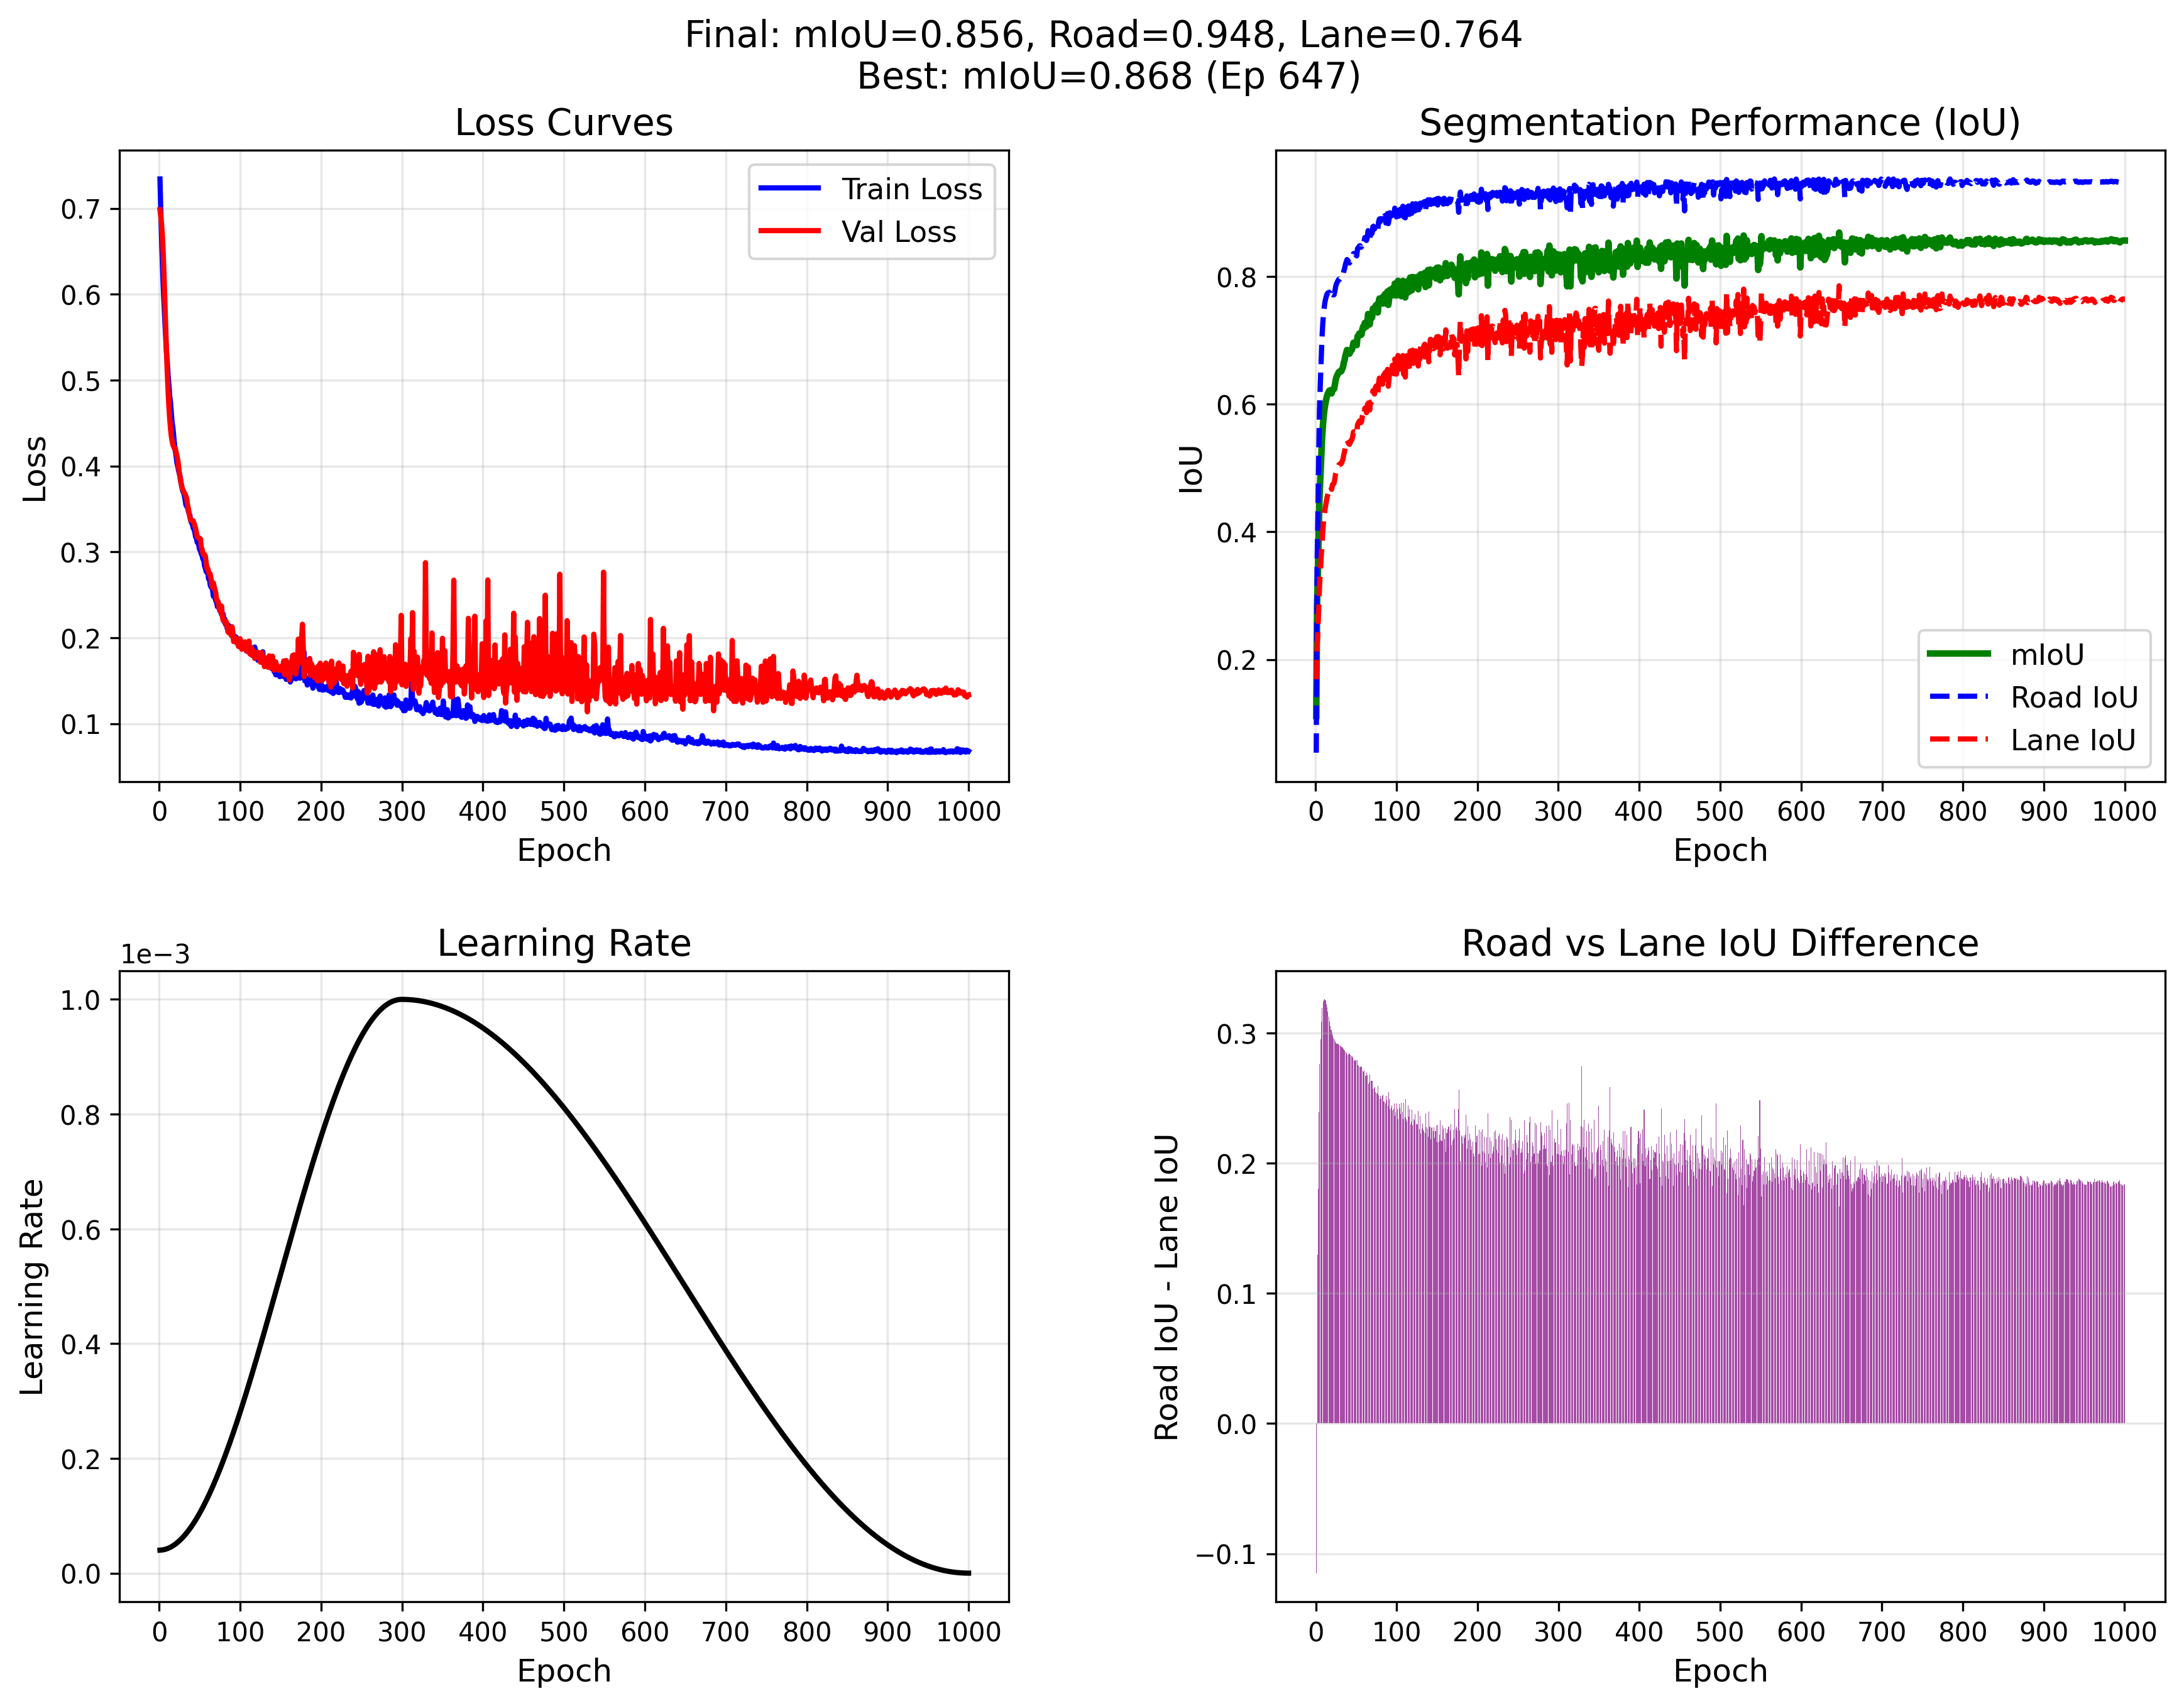
\includegraphics[width=0.8\textwidth]{figures/chapter3/fastscnn_training_analysis.png}
    \caption{FastSCNN模型训练分析}
    \label{fig:fastscnn_training}
\end{figure}

经过1000轮训练，模型在验证集上达到92.8\%的总体mIoU，其中道路区域IoU达94.3\%，非道路区域IoU为91.3\%。训练损失和验证损失均呈现稳定下降趋势，表明模型没有明显过拟合。值得注意的是，训练初期（约100轮）模型即表现出良好学习能力，随后性能增益逐渐平缓，符合深度学习模型的典型学习曲线。

在实际道路场景测试中，模型表现出良好鲁棒性，能有效识别不同光照条件下的可行驶区域，对复杂路况（如路面标记、树影和部分遮挡）也具有较强抗干扰能力。特别是在处理曝光不均和阴影区域时，FastSCNN比传统方法表现更为稳定。

结合车道线检测结果，FastSCNN语义分割输出为道路预行区域选取提供了可靠的语义约束，弥补了传统图像处理技术在复杂场景下的不足，为后续路径规划和决策系统提供高质量的环境感知输入。

\subsection{图像处理与语义分割叠加}

传统图像处理方法与深度学习语义分割技术各具优势：前者基于明确的几何和颜色特征，计算效率高且结果可解释性强，特别适合提取结构化特征如车道线；后者则能够理解复杂场景语义，对光照变化和路面纹理具有更强的鲁棒性。为最大化发挥两种技术的互补性，本研究设计了融合框架，实现车道线精确定位与可行驶区域可靠识别的双重目标。

融合过程采用基于空间关系的加权组合策略。首先，将FastSCNN语义分割结果与传统车道线检测进行空间对齐，确保两种结果在同一坐标系下比较。对于每个像素位置，系统会根据其与检测到的车道线的距离关系，动态调整传统方法与深度学习方法结果的权重。这种设计确保在车道线附近区域优先采用传统方法的精确边界定位，而在远离车道线的复杂区域则更依赖语义分割的全局理解能力。

图\ref{fig:fusion_comparison}展示了传统图像处理与融合方法的对比结果。可以清晰观察到，传统方法（图a）在车道线边界提供了精确定位，但在复杂路面纹理和光照变化区域存在不稳定性；融合结果（图b）则既保留了清晰的车道线边界，又提供了语义上连贯的可行驶区域表示，特别是在远处和光照不均区域表现出显著优势。

\begin{figure}[H]
    \centering
    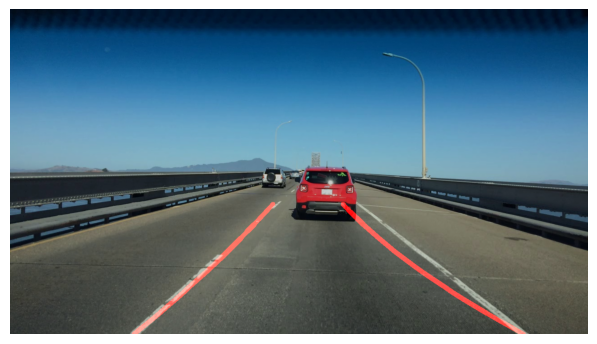
\includegraphics[width=0.48\textwidth]{figures/chapter3/compare_l.png}
    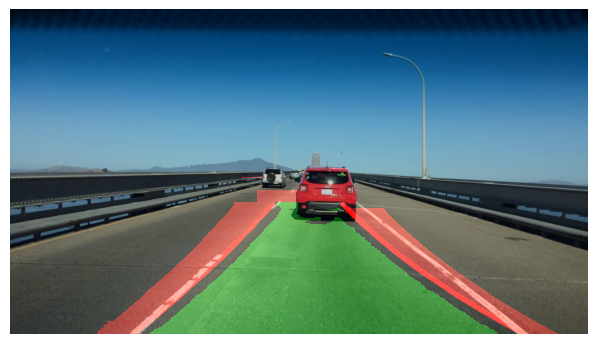
\includegraphics[width=0.48\textwidth]{figures/chapter3/compare_r.png}
    \begin{center}
    (a) 传统图像处理结果 \hspace{3cm} (b) 融合方法结果
    \end{center}
    \caption{图像处理与语义分割融合对比}
    \label{fig:fusion_comparison}
\end{figure}

通过实验观察，融合方法在多种场景下均表现出比单一方法更高的稳定性。特别是在处理光照不均、阴影区域和复杂路面纹理时，融合策略能够有效减少误识别情况，提高道路区域识别的整体准确性。同时，系统保持了可接受的实时性能，能够满足车载环境下的实时处理需求。

此融合框架为系统赋予了"双保险"机制——即使一种方法在特定条件下失效，另一种方法仍能提供有效输出。例如，在车道线模糊或被遮挡的区域，语义分割仍能给出合理的可行驶区域估计；而在光照极端或纹理混乱导致语义分割困难的情况下，几何特征明确的车道线检测能够提供可靠参考。这种互补设计对于安全关键型应用至关重要，确保了系统在多种环境条件下的可靠运行。

基于融合结果，系统能够更准确地界定安全的预行区域边界，为后续碰撞风险评估和轨迹规划提供可靠基础。这种集成方法不仅提高了系统的感知能力，也增强了决策的安全性和可靠性。


% ----------------------------------------------------------------------------------------------------------------------------------------------------------------------------------------------------------------------------------------------------------------------------------------------------------
\newpage
\renewcommand{\thefigure}{\thesection.\arabic{figure}}
\renewcommand{\thetable}{\thesection.\arabic{table}}
\renewcommand{\figurename}{图}
\setcounter{figure}{0} % 重置图表计数器
\setcounter{equation}{0} % 重置公式计数器

\section{监测障碍}
\subsection{障碍检测}
在自动驾驶系统中，准确识别和检测道路上的障碍物是保障行车安全的关键环节。障碍物检测系统需要实时识别包括行人、车辆、交通信号灯等各类道路元素，以便驾驶系统能够做出及时、准确的决策。本节将详细介绍基于深度学习的障碍物检测方法，包括数据集的预处理、目标检测模型的选择与训练、模型评估以及模型蒸馏技术的应用，以实现在保证检测精度的同时提高模型的推理速度。

采用YOLOv5系列模型作为基础检测框架，该系列模型以其出色的精度和实时性能在目标检测领域得到广泛应用。针对自动驾驶场景的特殊需求，对模型进行了针对性的优化和训练，以提高在道路场景中的检测能力。

\subsubsection{数据集预处理}
本研究使用BDD100K数据集进行模型训练和验证。BDD100K是一个大规模、多样化的驾驶视频数据集，包含10万张高分辨率图像，覆盖不同时间、天气条件和驾驶场景，为自动驾驶感知系统的研究提供了丰富的数据资源。

为了适应训练资源限制并提高训练效率，选择使用BDD100K数据集的一半数据进行训练和验证。数据预处理主要包括以下步骤：

\begin{circledlist}
    \item 图像筛选与分割：将原始数据集按照训练集和验证集进行划分，并随机抽样以获取所需比例的数据。
    \item 标注格式转换：将BDD100K原始的JSON格式标注转换为YOLO模型所需的标准格式。
    \item 类别映射：将原始数据集中的多类别目标映射为两大类——活动障碍物（包括行人、骑车人、汽车等）和交通信号（包括交通灯和交通标志）。
    \item 坐标归一化：将目标边界框的坐标从像素值转换为归一化的相对值。
\end{circledlist}

通过上述预处理，将BDD100K数据集转换为适合YOLOv5模型训练的格式，并创建了相应的配置文件。数据集中的目标被划分为两类：活动障碍物（类别0）和交通信号（类别1），这种分类方式有助于模型更好地理解和区分道路场景中不同类型的障碍物。

\subsubsection{障碍目标检测}

在经过充分训练后，将训练好的模型应用于实际道路场景的障碍物检测任务。图\ref{fig:detection}展示了该模型在不同场景下的检测效果。

\begin{figure}[H]
    \centering
    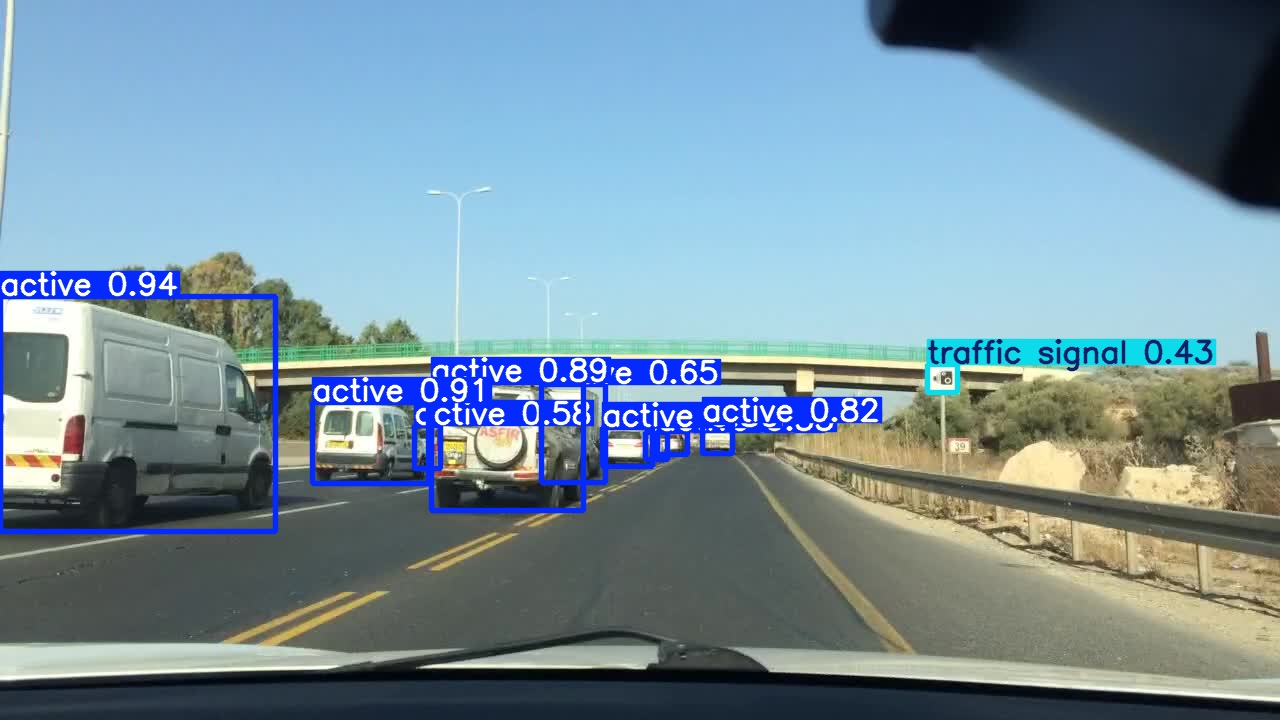
\includegraphics[width=0.45\textwidth]{figures/chapter4/a.jpg}
    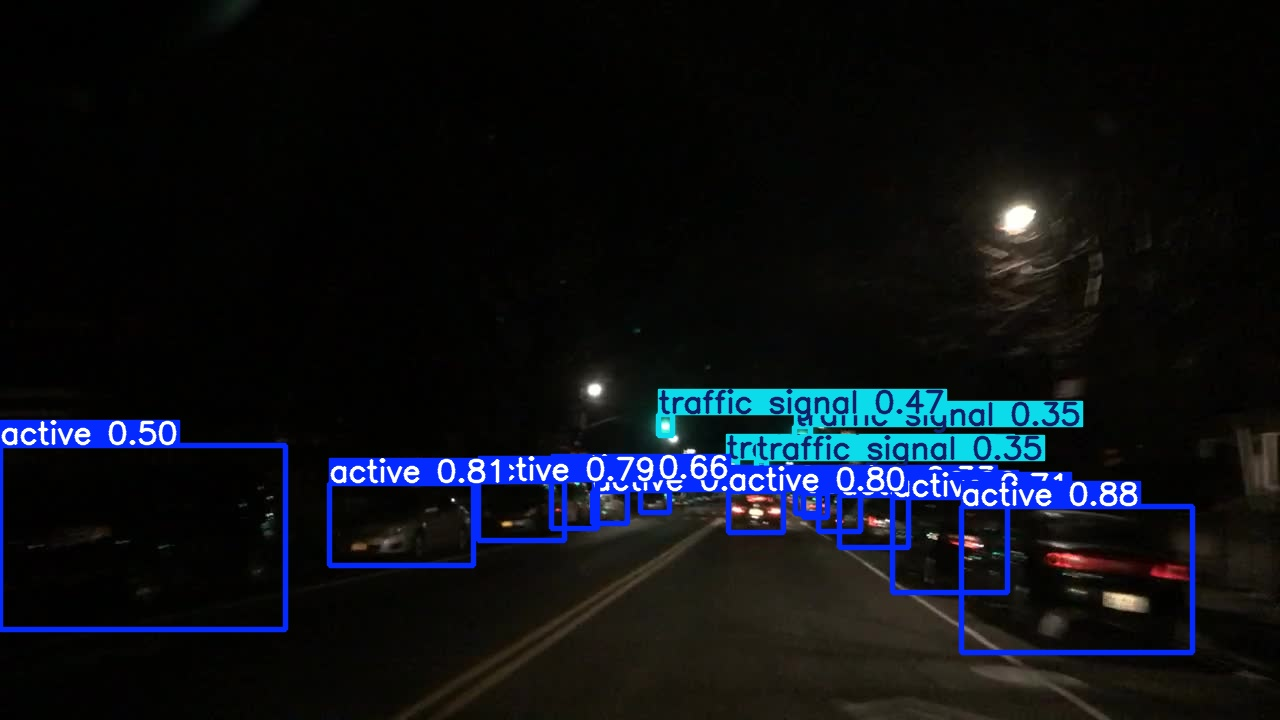
\includegraphics[width=0.45\textwidth]{figures/chapter4/b.jpg}

    \caption{(a) 城市道路检测效果 (b) 复杂环境下检测效果 \\目标检测效果}
    \label{fig:detection}
\end{figure}

从检测结果可以看出，的模型能够准确识别和定位道路场景中的各类障碍物。模型成功检测到了城市道路环境中的多辆车辆，并给出了准确的边界框和置信度得分，展示了模型在更为复杂的交通环境中的表现，能够同时检测到车辆、行人以及交通信号灯等多种目标，表明模型具有较强的鲁棒性和适应性。

检测结果中，每个目标都标记了相应的类别和检测置信度。活动障碍物以一种颜色标记，而交通信号以另一种颜色标记，通过对动态障碍物的检测和跟踪可以有效降低事故发生概率。

\subsubsection{模型训练与评估}
在模型训练中，采用了Ultralytics提供的YOLOv5框架对模型进行训练。训练过程中，采用了以下策略：

\begin{halfparlist}
    \item 数据增强：应用随机裁剪、旋转、缩放、亮度调整等增强技术，提高模型对不同场景的适应能力。
    \item 学习率调度：采用余弦退火策略动态调整学习率，以实现更好的收敛效果。
    \item 批量归一化：在网络各层之间应用批量归一化，加速训练过程并提高模型稳定性。
    \item 早停机制：监控验证集上的性能，防止过拟合。
\end{halfparlist}

图\ref{fig:training_validation_curves}展示了模型在训练过程中的各项性能指标变化趋势。

\begin{figure}[H]
    \centering
    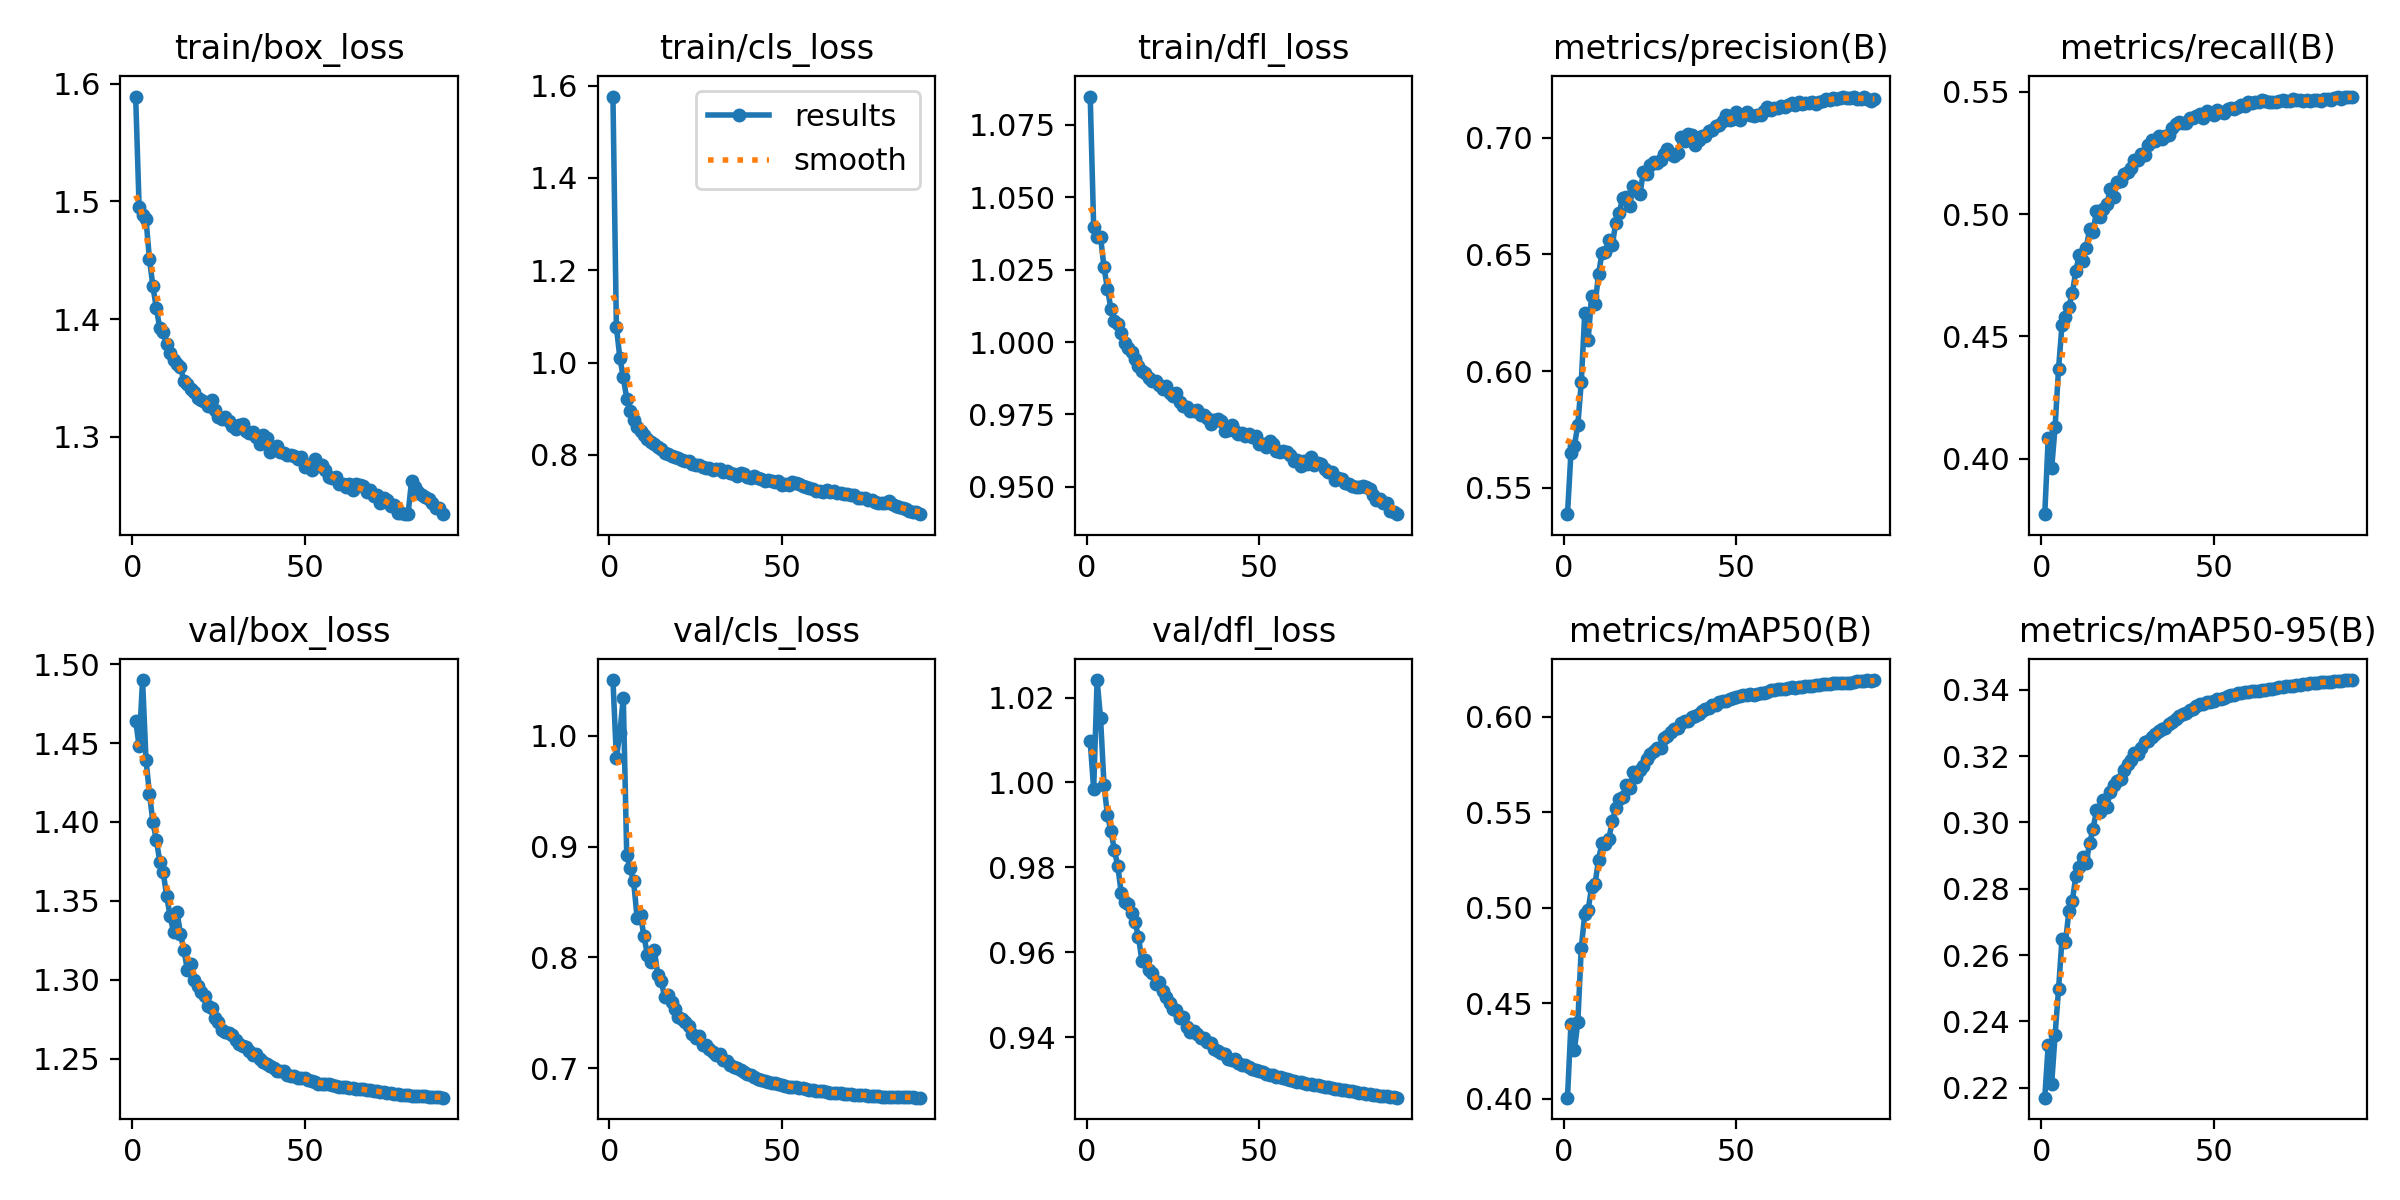
\includegraphics[width=1\textwidth]{figures/chapter4/val.png}
    \caption{模型训练验证性能曲线}
    \label{fig:training_validation_curves}
\end{figure}

从性能曲线可以观察到，随着训练轮次的增加，模型的mAP、精确率和召回率均呈现稳定上升趋势，并最终趋于收敛。这表明模型能够有效学习数据集中的特征分布，并在验证集上展现出良好的泛化能力。特别是在训练后期，模型的mAP@0.5指标达到了61\%以上、mAP@0.5:0.95达到0.34以上，表明在IoU阈值为0.8的条件下，该模型具有较高的检测准确性。

为全面评估目标检测模型性能，采用了以下几个关键指标：

\begin{parlist}
    \item 精确率(Precision)：表示在所有被预测为正类的样本中，真正为正类的比例。
    \begin{equation}
        \text{Precision} = \frac{\text{TP}}{\text{TP} + \text{FP}}
    \end{equation}

    \item 召回率(Recall)：表示在所有真实为正类的样本中，被正确预测的比例。
    \begin{equation}
        \text{Recall} = \frac{\text{TP}}{\text{TP} + \text{FN}}
    \end{equation}

    \item F1分数：精确率和召回率的调和平均值，提供了一个平衡的性能度量。
    \begin{equation}
        \text{F1} = 2 \cdot \frac{\text{Precision} \cdot \text{Recall}}{\text{Precision} + \text{Recall}}
    \end{equation}

    \item 平均精度(AP)：在不同召回率水平下精确率的平均值，对每个类别单独计算。

    \item 平均精度均值(mAP)：所有类别AP的平均值，通常使用特定的IoU(交并比)阈值，如mAP@0.5或mAP@0.5:0.95。

    \item IoU(交并比)：是评估预测边界框与真实边界框重叠程度的关键指标：
\end{parlist}

\begin{equation}
IoU(A, B) = \frac{A \cap B}{A \cup B}
\end{equation}

\subsubsection{模型蒸馏及量化}

\begin{parlist}


\item 模型蒸馏（Model Distillation）

模型蒸馏是一种知识压缩技术。它通过将大型且性能优越的教师模型中的知识迁移到结构更为精简的学生模型，实现模型的轻量化与高效推理。在蒸馏过程中，学生模型不仅学习传统的硬标签（ground-truth label），还通过最小化与教师模型输出的软标签（soft label，通常为softmax概率分布）之间的差异，获得更多关于类别间关系的信息。常用的损失函数包括交叉熵损失和Kullback-Leibler散度。

\item 模型量化（Model Quantization）

模型蒸馏是一种常用的模型压缩与加速技术。它通过将模型参数和计算从高精度（如32位浮点数）转换为低精度（如8位整数），有效减少模型存储空间和推理时的计算资源消耗。量化不仅显著降低了模型的存储和带宽需求，还提升了模型在边缘设备上的推理速度。常见的量化方法包括静态量化（Post-Training Static Quantization）和动态量化（Dynamic Quantization）：

\begin{halfparlist}
    \item 静态量化

    在模型推理前，利用一部分校准数据对模型的权重和激活进行量化参数的统计和校准，将其统一映射为低精度格式。该方法适用于YOLOv5等目标检测模型，能够在保证精度的前提下大幅提升推理效率。

    \item 动态量化

    在推理过程中，动态地将部分权重或激活从高精度转换为低精度。该方法适用于对延迟和存储要求较高、但对精度损失容忍度较高的场景。动态量化通常对模型权重进行量化，而激活则在推理时动态处理。

    \end{halfparlist}

\end{parlist}

在YOLOv5模型中，量化通常结合PyTorch等深度学习框架实现，支持对卷积层、全连接层等关键算子的量化。通过量化，YOLOv5模型能够在移动端、嵌入式等资源受限设备上实现高效部署，同时保持较好的检测性能。

本文采用基于YOLO的知识蒸馏（Knowledge Distillation, KD）方法，以提升轻量级检测模型的性能。首先，训练一个结构复杂、性能优越的教师模型（YOLOv5s-ultralytics，YOLOv5su），随后利用其输出指导学生模型（YOLOv5n-ultralytics，YOLOv5nu）的训练。
训练过程中，学生模型不仅最小化与真实标签的常规检测损失，还通过最小化与教师模型输出之间的蒸馏损失，实现知识迁移。
蒸馏损失包括边界框、置信度和分类输出的差异，采用均方误差（MSE）和Kullback-Leibler散度（KL）进行度量。为平衡检测损失与蒸馏损失的贡献，引入余弦退火策略动态调整蒸馏损失权重。
最后，通过对学生模型的静态量化，保证模型精度的同时，提升推理效率，结合tensorflow lite micro（tflite-micro）库，可对模型进行边缘部署。

损失函数定义如下：
\begin{equation}
L = L_{\text{det}} + \lambda_{\text{KD}} \cdot L_{\text{KD}}
\end{equation}

其中，$L_{\text{det}}$为学生模型的常规检测损失，$L_{\text{KD}}$为蒸馏损失，$\lambda_{\text{KD}}$为蒸馏损失权重，采用余弦退火策略动态调整：

\begin{equation}
\lambda_{\text{KD}}(e) = \lambda_{\text{final}} + 0.5 \cdot (\lambda_{\text{init}} - \lambda_{\text{final}}) \cdot \left[1 + \cos\left(\frac{\pi \cdot e}{E}\right)\right]
\end{equation}

其中，$e$为当前epoch，$E$为总epoch数，$\lambda_{\text{init}}$和$\lambda_{\text{final}}$分别为初始和最终蒸馏权重。

\begin{align}
L_{\text{box}} &= \text{MSE}(S_{\text{box}}, T_{\text{box}}) \\
L_{\text{conf}} &= \text{KL}\left(\text{Softmax}\left(\frac{T_{\text{conf}}}{T}\right) \Big\| \text{Softmax}\left(\frac{S_{\text{conf}}}{T}\right)\right) \cdot T^2 \\
L_{\text{cls}} &= \text{KL}\left(\text{Softmax}\left(\frac{T_{\text{cls}}}{T}\right) \Big\| \text{Softmax}\left(\frac{S_{\text{cls}}}{T}\right)\right) \cdot T^2
\end{align}

最终蒸馏损失为：
\begin{equation}
L_{\text{KD}} = L_{\text{box}} + L_{\text{conf}} + L_{\text{cls}}
\end{equation}

整体流程如图\ref{fig:distill-flow}所示

\begin{figure}[H]
    \centering
    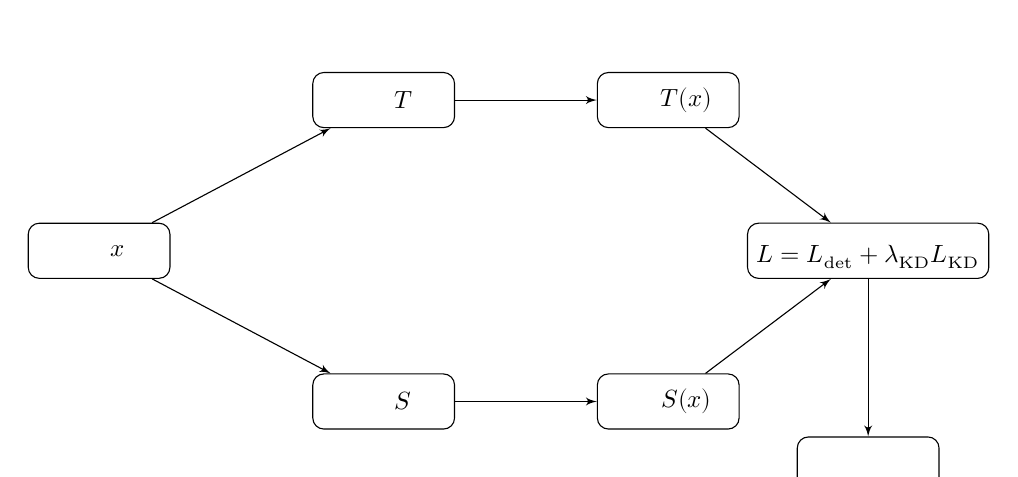
\begin{tikzpicture}[
        node distance=1.2cm and 1.8cm,
        every node/.style={rounded corners, draw, align=center, minimum width=1.8cm, minimum height=0.7cm, font=\small},
        >=latex'
    ]
        % Nodes
        \node (input) {输入图像 $x$};
        \node (teacher) [above right=of input] {教师模型 $T$};
        \node (student) [below right=of input] {学生模型 $S$};
        \node (t_out) [right=of teacher] {教师输出 $T(x)$};
        \node (s_out) [right=of student] {学生输出 $S(x)$};
        \node (loss) [right=1cm of $(t_out)!0.5!(s_out)$, minimum width=2.8cm] {损失计算\\$L = L_{\text{det}} + \lambda_{\text{KD}} L_{\text{KD}}$};
        \node (opt) [below=2cm of loss] {反向传播优化};

        % Arrows
        \draw[->] (input) -- (teacher);
        \draw[->] (input) -- (student);
        \draw[->] (teacher) -- (t_out);
        \draw[->] (student) -- (s_out);
        \draw[->] (t_out) -- (loss);
        \draw[->] (s_out) -- (loss);
        \draw[->] (loss) -- (opt);
    \end{tikzpicture}
    \caption{知识蒸馏训练流程}
    \label{fig:distill-flow}
\end{figure}


虽然YOLOv5nu模型的参数量仅为YOLOv5su的三分之一，但通过蒸馏，仅需约100轮训练，即可快速收敛至教师模型95\%的检测精度，实现了显著的模型压缩。

下文对教师模型（YOLOv5su）、蒸馏后的学生模型（YOLOv5nu-蒸馏）和未经蒸馏训练的学生模型（YOLOv5nu-原始）进行了全面性能比较。

从图\ref{fig:processing_time}可以看出，蒸馏后的YOLOv5nu模型相较于原始教师模型YOLOv5su，推理速度提升至其171\%（在Kaggle单GPU T4 15G环境下测试）。这一速度提升对于自动驾驶系统的实时决策至关重要，使系统能够更快响应环境变化。

\begin{figure}[H]
    \centering
    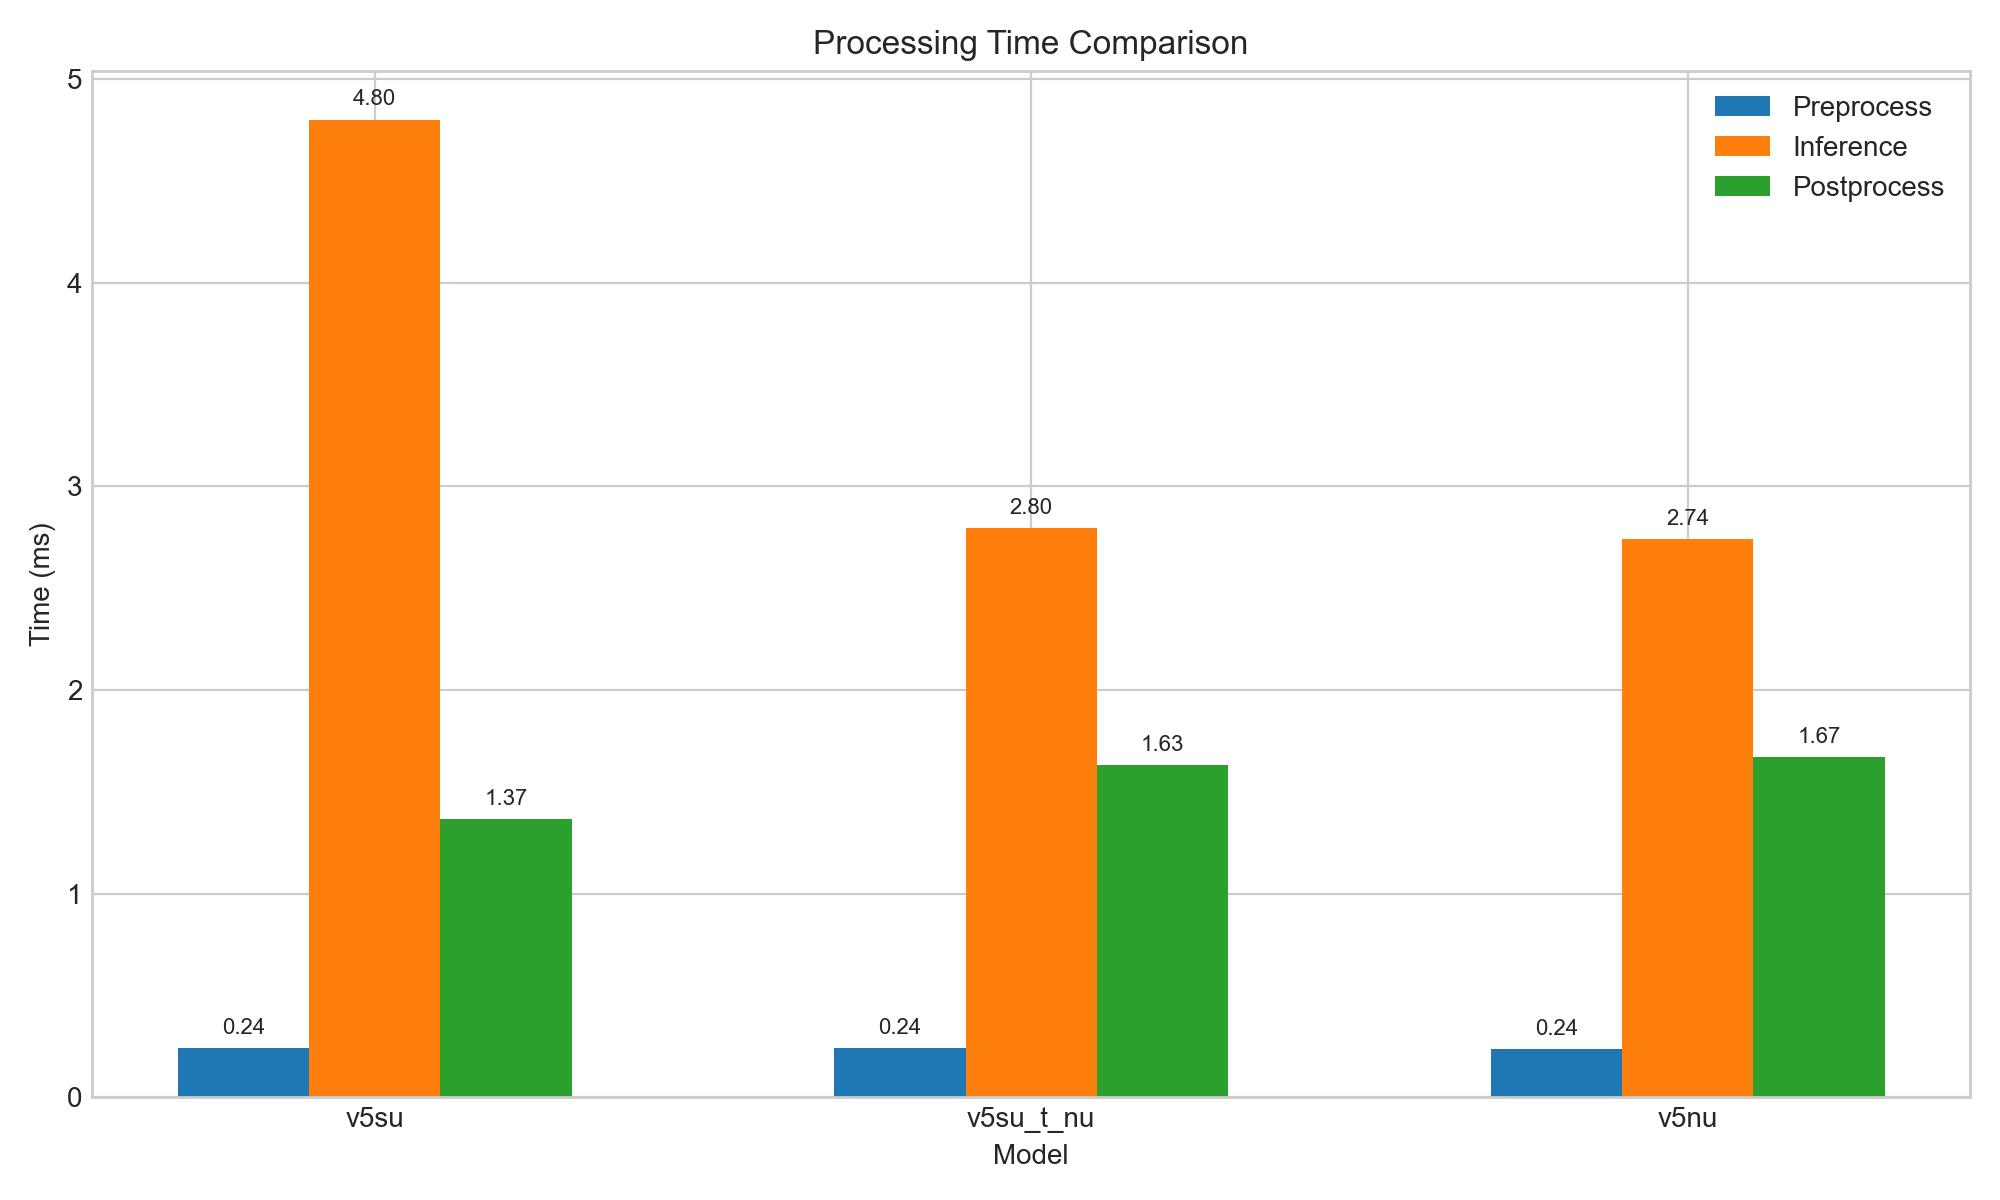
\includegraphics[width=\textwidth]{figures/chapter4/ptc.png}
    \caption{处理速度对比图}
    \label{fig:processing_time}
\end{figure}

在智能驾驶等对处理速度要求严格的场景，FPS尤为重要。如图\ref{fig:fps_comparison}所示，蒸馏后的YOLOv5nu模型在保留高处理速度的同时，也较好地保持了YOLOv5su的检测精度。

\begin{figure}[H]
    \centering
    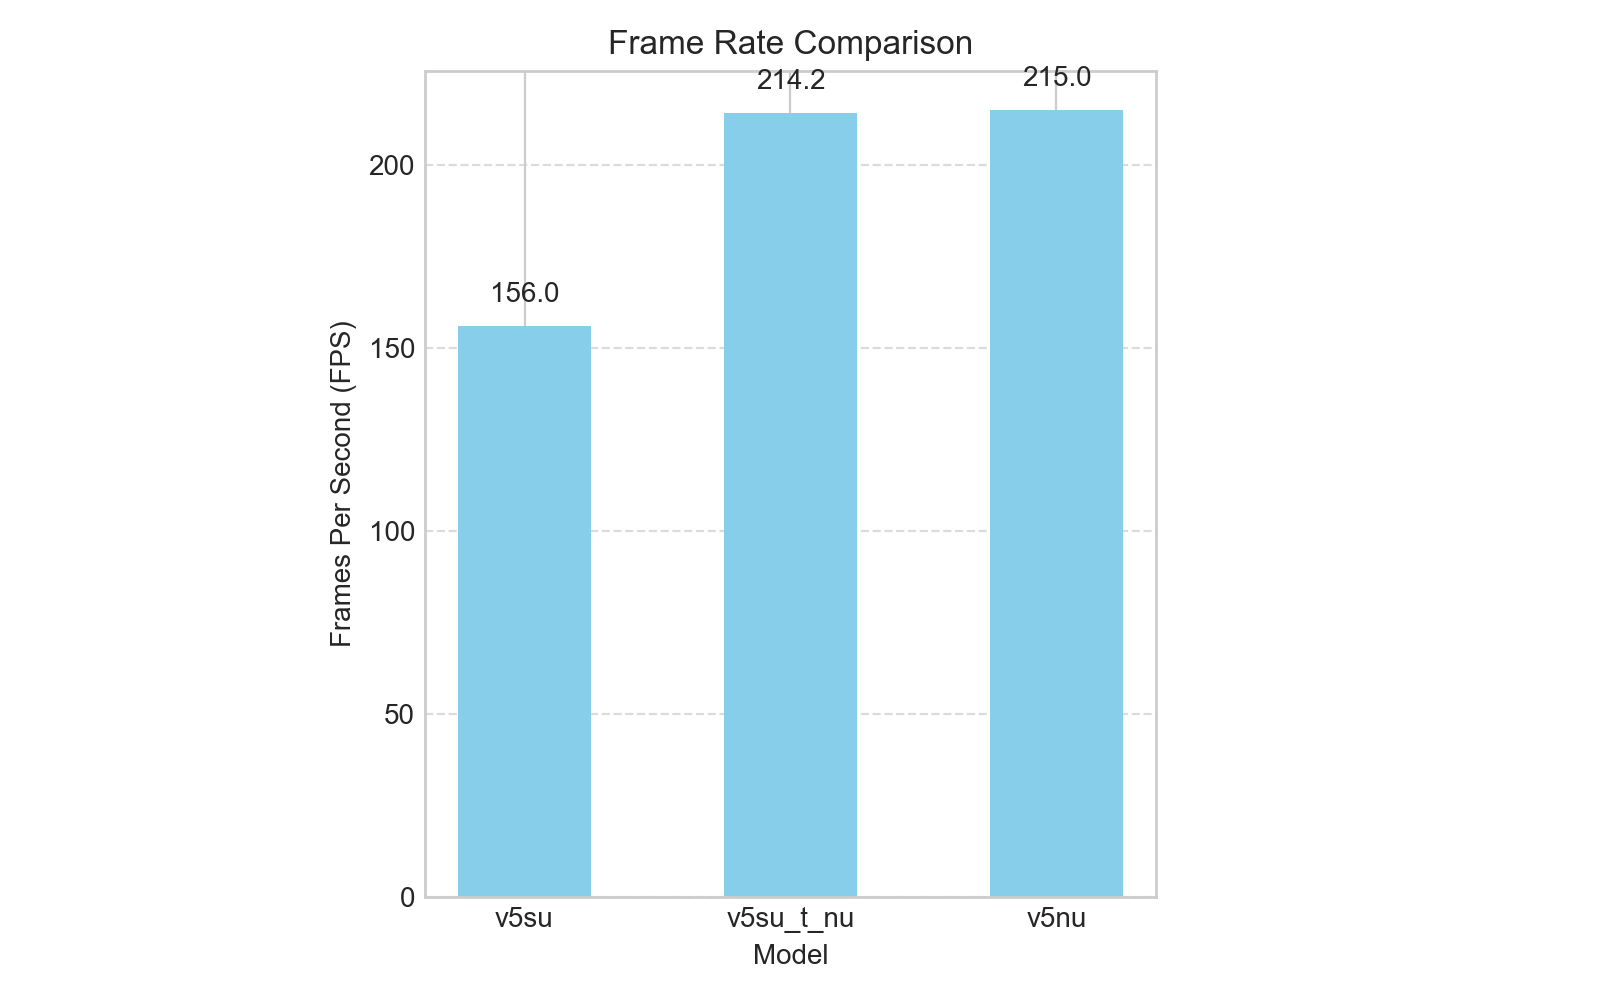
\includegraphics[width=0.8\textwidth]{figures/chapter4/fps.png}
    \caption{帧率对比图}
    \label{fig:fps_comparison}
\end{figure}

图\ref{fig:accuracy_loss_comparison}展示了三种模型在精度和损失函数方面的对比。

\begin{figure}[H]
    \centering
    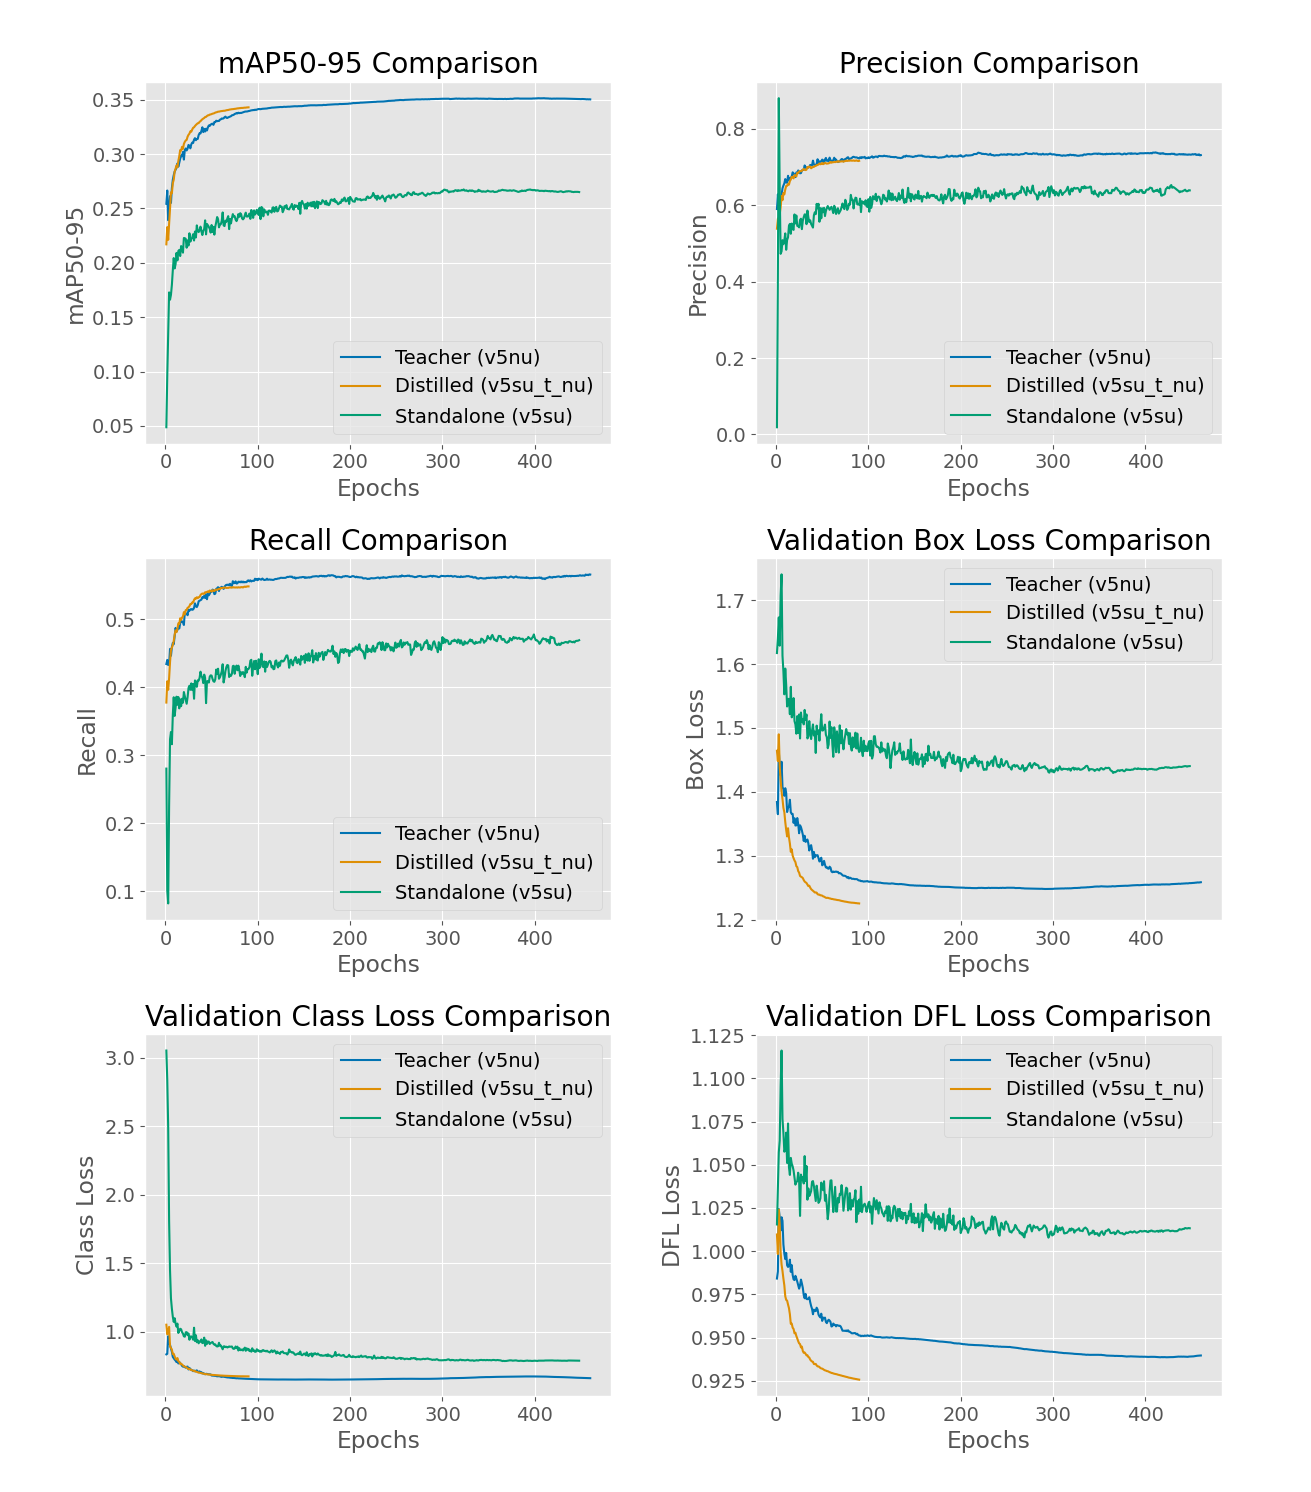
\includegraphics[width=1\textwidth]{figures/chapter4/three_compare.png}
    \caption{模型精度和损失对比}
    \label{fig:accuracy_loss_comparison}
\end{figure}

可以看出，虽然蒸馏后的YOLOv5nu模型参数量大幅减少，但其检测精度仅略低于教师模型YOLOv5su，且明显优于未经蒸馏的YOLOv5nu-原始模型。这表明知识蒸馏有效地将教师模型的表示能力转移到了更小的学生模型中。

图\ref{fig:comprehensive_performance}进一步展示了三种模型在各项关键性能指标上的最终表现。

\begin{figure}[H]
    \centering
    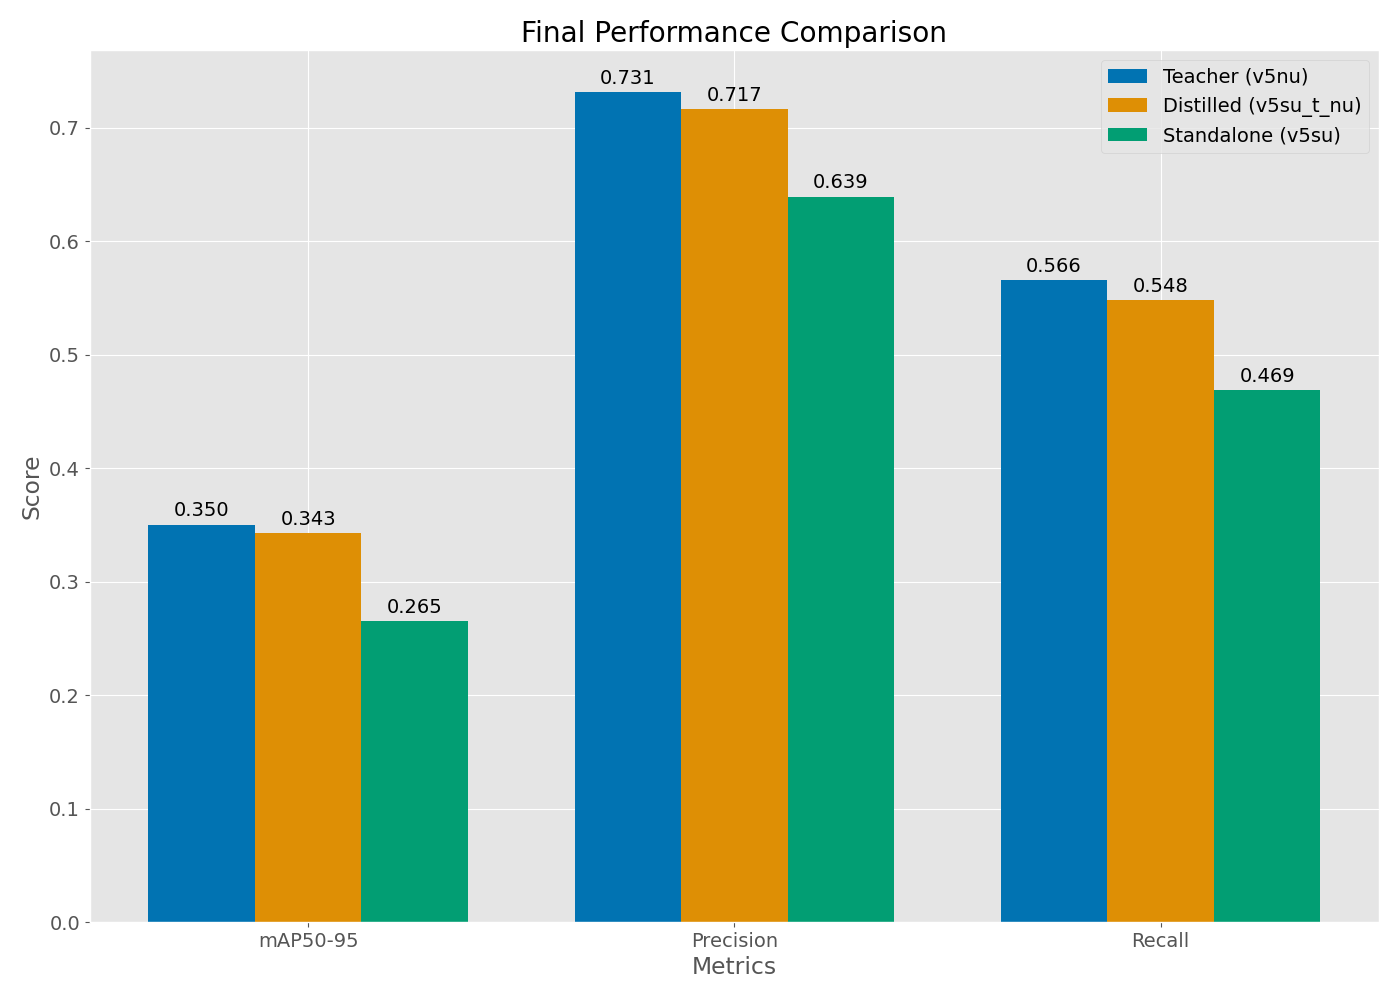
\includegraphics[width=1\textwidth]{figures/chapter4/final_performance.png}
    \caption{模型综合性能比较}
    \label{fig:comprehensive_performance}
\end{figure}

如图\ref{fig:comprehensive_performance}所示，在mAP、精确率、召回率和F1分数等关键指标上，蒸馏后的YOLOv5nu模型均达到了接近教师模型的水平，同时在模型大小和推理速度方面具有显著优势。


尤其是在自动驾驶场景下最为关注的mAP@0.5指标，蒸馏后模型达到了教师模型97.6\%以上的性能，而直接训练的YOLOv5nu模型仅为教师模型的76.1\%，提升了21.5\%。这充分说明，知识蒸馏能够在保持较高精度的同时，大幅降低模型复杂度和推理时间，满足自动驾驶系统对实时性和资源效率的高要求。


综上所述，通过知识蒸馏、量化技术，成功实现了模型的轻量化，为自动驾驶系统中的障碍物检测任务提供了一个高效、实用的解决方案。这种优化后的模型更适合部署在计算资源有限的车载环境中，能够支持系统进行实时、准确的障碍物检测和避障决策。


% 000
\subsection{障碍跟踪}
\subsubsection{改进的DeepSORT框架}

\begin{parlist}


\item 检测关联机制


DeepSORT的核心创新在于其级联关联策略，该策略将目标的外观特征与运动状态信息融合，构建多元相似度度量机制。此方法在计算关联代价时，同时考虑外观相似性（通过深度特征提取）和运动连续性（通过卡尔曼滤波预测）。
DeepSORT的系统架构如图\ref{fig:deepsort}所示，该架构包括了特征提取模块、卡尔曼滤波模块和关联模块。特征提取模块用于提取目标的深度特征，卡尔曼滤波模块用于预测目标的运动状态，关联模块用于计算目标的关联代价并进行关联决策。
\begin{figure}[H]
\centering
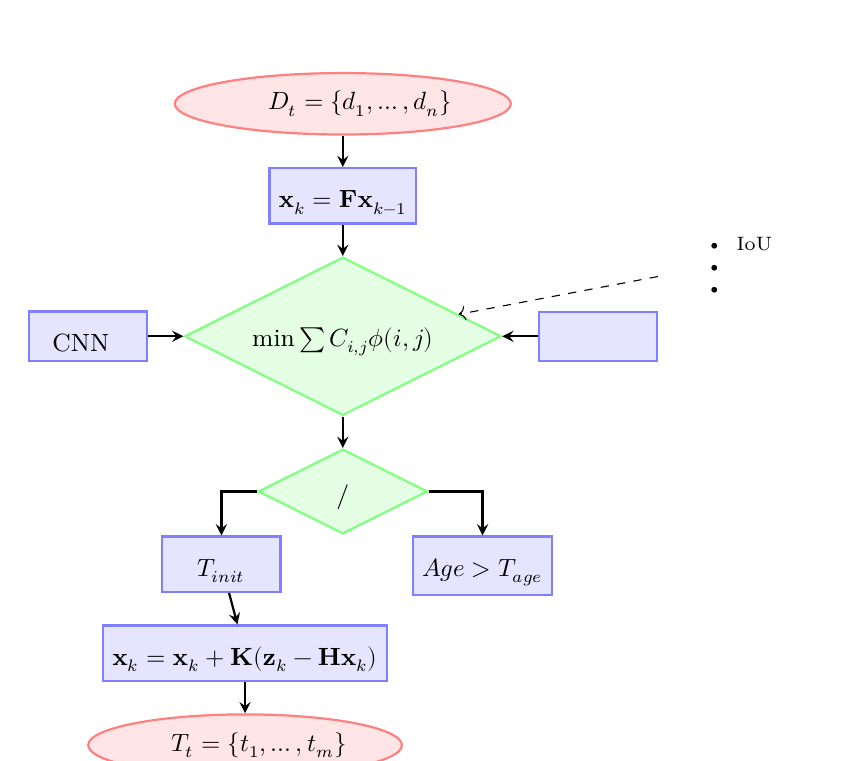
\begin{tikzpicture}[
node distance=4mm,
module/.style={rectangle, draw=blue!50, fill=blue!10, thick, minimum width=15mm, minimum height=3mm, align=center, font=\small},
decision/.style={diamond, draw=green!50, fill=green!10, thick, aspect=2, align=center, font=\small},
data/.style={ellipse, draw=red!50, fill=red!10, thick, align=center, font=\small},
arrow/.style={->, >=stealth, thick}
]

% 节点定义
\node[data] (input) {检测框序列$D_t=\{d_1,\ldots,d_n\}$};
\node[module, below=of input] (kf_predict) {卡尔曼滤波预测\\$\mathbf{x}_k = \mathbf{F}\mathbf{x}_{k-1}$};
\node[decision, below=of kf_predict] (association) {级联匹配\\$\min\sum C_{i,j}\phi(i,j)$};
\node[module, left=of association, xshift=-0.5mm] (appearance) {外观特征提取\\CNN模型};
\node[module, right=of association, xshift=0.5mm] (motion) {运动特征计算\\马氏距离};
\node[decision, below=of association] (unmatched) {未匹配\\检测/轨迹};
\node[module, below left=of unmatched, xshift=0.5mm] (new_track) {创建新轨迹\\$T_{init}$};
\node[module, below right=of unmatched, xshift=0.5mm] (delete_track) {删除旧轨迹\\$Age>T_{age}$};
\node[module, below=of new_track, xshift=3mm] (update) {状态更新\\$\mathbf{x}_k = \mathbf{x}_k + \mathbf{K}(\mathbf{z}_k-\mathbf{H}\mathbf{x}_k)$};
\node[data, below=of update] (output) {跟踪结果$T_t=\{t_1,\ldots,t_m\}$};

% 连接路径
\draw[arrow] (input) -- (kf_predict);
\draw[arrow] (kf_predict) -- (association);
\draw[arrow] (appearance) -- (association);
\draw[arrow] (motion) -- (association);
\draw[arrow] (association) -- (unmatched);
\draw[arrow] (unmatched) -| node[above left, font=\scriptsize] {新检测} (new_track);
\draw[arrow] (unmatched) -| node[above right, font=\scriptsize] {失配轨迹} (delete_track);
\draw[arrow] (new_track) -- (update);
\draw[arrow] (update) -- (output);

% 侧边注释 - 移动到了更合适的位置
\node[text width=1.8cm, font=\scriptsize, anchor=west] at (4,-2) (note1) {
匹配策略：
\begin{itemize}[noitemsep,topsep=0pt,parsep=0pt,partopsep=0pt]
\item IoU关联
\item 外观相似度
\item 运动一致性
\end{itemize}
};

\draw[->, dashed] (note1) -- (association);

\end{tikzpicture}
\caption{DeepSORT算法框架}
\label{fig:deepsort}
\end{figure}

具体而言，算法通过加权组合马氏距离（衡量运动状态差异）和余弦距离（衡量外观特征差异）来评估检测框与已有轨迹的匹配程度。在车载场景中，运动信息权重通常设为0.7，外观特征权重设为0.3，这种配置表现最佳。

\item 卡尔曼滤波预测

DeepSORT使用线性卡尔曼滤波器对目标运动状态进行建模和预测，这是保障算法稳定性的关键。卡尔曼滤波包含两个主要阶段：

\begin{circledlist}
    \item 预测阶段：根据上一时刻的状态估计当前时刻状态
    \item 更新阶段：结合实际观测数据对预测状态进行修正
\end{circledlist}

在车辆跟踪应用中，状态向量包含边界框中心坐标、宽高比、高度及其对应的速度分量。这种设计使系统能够在检测暂时丢失的情况下，仍然维持对目标位置的合理估计，有效应对短时遮挡场景。

\item 轨迹管理策略

DeepSORT采用三态轨迹生命周期管理机制，如图\ref{fig:track_lifecycle}所示，包括暂存(Tentative)、确认(Confirmed)和删除(Deleted)三种状态：

\begin{figure}[H]
\centering
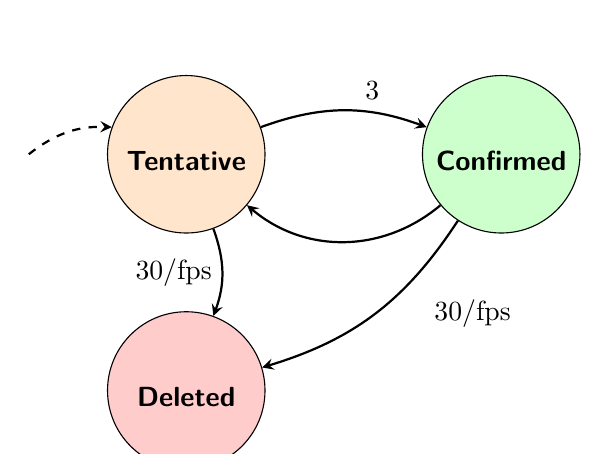
\begin{tikzpicture}[
    node distance=4cm,
    state/.style={circle, draw, minimum size=2cm, font=\sffamily\bfseries},
    arrow/.style={->, >=stealth, thick, bend left=20}
]

% 定义三个状态节点
\node[state, fill=orange!20, align=center] (tentative) {暂存\\Tentative};
\node[state, fill=green!20, right of=tentative, align=center] (confirmed) {确认\\Confirmed};
\node[state, fill=red!20, below of=tentative, yshift=1cm, align=center] (deleted) {删除\\Deleted};

% 添加状态转换箭头
\draw[arrow] (tentative) to node[above] {连续匹配 ≥ 3} (confirmed);
\draw[arrow] (tentative) to node[left] {未匹配 ≥ 30/fps} (deleted);
\draw[arrow] (confirmed) to node[right] {未匹配 ≥ 30/fps} (deleted);
\draw[arrow] (confirmed) to[bend left=40] node[below] {新检测} (tentative);

% 添加初始箭头
\draw[arrow, dashed] (-2, 0) to node[above] {新检测} (tentative);

\end{tikzpicture}
\caption{轨迹状态转换图}
\label{fig:track_lifecycle}
\end{figure}

此机制有效过滤短期误检，同时保持对长期稳定目标的连续跟踪：

\begin{circledlist}
    \item 新检测首先被标记为"暂存"状态
    \item 连续匹配3次后升级为"确认"状态
    \item 长时间未匹配（通常为30/fps帧）的轨迹被标记为"删除"状态
\end{circledlist}

通过这种状态管理机制，DeepSORT能够维持稳定的跟踪ID，减少ID切换频率，提高跟踪连续性。

\item 匹配算法优化

为解决检测框与轨迹的最优匹配问题，DeepSORT采用匈牙利算法(Hungarian Algorithm)求解全局最优分配方案。匹配过程分两阶段执行：

\begin{circledlist}
    \item 基于外观特征和运动状态匹配确认轨迹
    \item 仅基于IoU匹配剩余的检测框和短期轨迹
\end{circledlist}

这种级联匹配策略优先处理高质量轨迹，有效提高了密集场景下的匹配精度，特别是对于部分遮挡的车辆。

尽管原始DeepSORT在行人跟踪领域表现优异，但直接应用于车载场景时存在三个主要问题：特征提取模型不匹配、运动模型过于简化以及ID切换频繁。

\end{parlist}


\subsubsection{卡尔曼滤波器}

卡尔曼滤波器在车载障碍物跟踪中扮演着关键角色，通过结合运动模型和观测数据，为目标位置提供最优估计。本研究实现了针对车载环境优化的线性卡尔曼滤波器。

\begin{parlist}


\item 状态表示与运动模型

卡尔曼滤波的实现采用8维状态向量：

\begin{equation}
\mathbf{x} = [x, y, w, h, v_x, v_y, v_w, v_h]^T
\end{equation}

其中$(x, y)$表示目标中心坐标，$(w, h)$表示目标宽高，$(v_x, v_y)$表示中心点速度，$(v_w, v_h)$表示尺寸变化率。

状态转移矩阵$\mathbf{F}$采用匀速运动模型：

\begin{equation}
\label{eq:kalman_f}
\mathbf{F} =
\begin{bmatrix}
\mathbf{I}_4 & \Delta t \cdot \mathbf{I}_4 \\
\mathbf{0}_4 & \mathbf{I}_4
\end{bmatrix}
\end{equation}

其中$\mathbf{I}_4$为$4 \times 4$单位矩阵，$\Delta t$为帧间时间间隔。

\item 噪声调整与车速自适应

标准卡尔曼滤波器在应对车辆速度变化时面临挑战，因此引入了基于车速的过程噪声自适应机制：

\begin{equation}
\mathbf{Q}(v) = \mathbf{Q}_0 \cdot (1 + \alpha \cdot \|v\|)
\end{equation}

其中$\mathbf{Q}_0$为基础噪声协方差，$v$为估计速度向量，$\alpha$为调整系数。通过这种方式，系统对高速移动物体采用更大的过程噪声，提高跟踪鲁棒性。

\item 更新机制与平滑处理

为平滑跟踪结果，在测量更新阶段采用指数移动平均(EMA)滤波器：

\begin{equation}
\hat{\mathbf{x}}_t = \alpha \cdot \mathbf{z}_t + (1-\alpha) \cdot \hat{\mathbf{x}}_{t-1}
\end{equation}

其中$\hat{\mathbf{x}}_t$为更新后状态，$\mathbf{z}_t$为当前观测，$\alpha$为平滑系数。

特定优化后的卡尔曼滤波器，能够在资源受限的平台，保持较为理想的精度和效率，同时保持较低的计算开销。

\end{parlist}


\subsubsection{匈牙利算法级联匹配}

在目标跟踪过程中，将新检测框与现有轨迹进行关联是关键挑战。采用匈牙利算法进行全局最优匹配，并引入级联匹配策略以提高复杂场景下的关联精确度。

\begin{parlist}
\item 代价矩阵构建

匹配过程首先构建代价矩阵$\mathbf{C}$，其中元素$c_{ij}$表示第$i$个轨迹与第$j$个检测之间的关联代价：

\begin{equation}
c_{ij} = \lambda \cdot d_{motion}(i,j) + (1-\lambda) \cdot d_{appearance}(i,j)
\end{equation}

其中$d_{motion}$为运动距离（基于IoU计算），$d_{appearance}$为表观距离，$\lambda$为权重系数（在的实现中设为1.0，仅使用IoU距离）。

\item 贪心匹配算法实现

为适应资源受限嵌入式平台，采用贪心匹配策略替代标准匈牙利算法，在保证性能的同时显著降低计算复杂度。

\item 级联匹配策略

为处理车载场景中常见的遮挡和密集目标，实现了基于轨迹质量的级联匹配策略：

\begin{circledlist}
    \item 首先匹配高质量轨迹（连续跟踪帧数多的）
    \item 再匹配中等质量轨迹
    \item 最后处理低质量轨迹和新初始化轨迹
\end{circledlist}

这种策略确保稳定轨迹获得优先匹配权，从而提高系统在复杂场景的鲁棒性。

\item 阈值动态调整

引入IoU阈值的动态调整机制，根据目标大小、速度和跟踪历史进行自适应设置：

\begin{equation}
\tau_{iou}(v, a) = \tau_0 \cdot e^{-\beta \cdot \|v\| \cdot a}
\end{equation}

其中$\tau_0$为基础阈值（0.7），$v$为估计速度，$a$为目标面积，$\beta$为调整系数。这使系统能够为快速移动的小目标使用更宽松的匹配标准。

\end{parlist}

\subsubsection{特征度量}

在资源受限的嵌入式平台上实现高效的特征表示和度量是一个显著挑战。开发了一套轻量级特征度量方法，适合嵌入式低功耗设备。
\begin{parlist}


\item 外观特征简化

考虑到在嵌入式设备运行的资源局限，及在道路使用上的时空连贯性，本文简化了传统DeepSORT中基于深度学习的特征提取过程，改用更高效的几何和运动特征：

\begin{halfparlist}
    \item 边界框宽高比：$r = w/h$
    \item 尺寸一致性：$s_{cons} = \min(w_1/w_2, w_2/w_1) \cdot \min(h_1/h_2, h_2/h_1)$
    \item 运动一致性：通过速度向量余弦相似度计算
\end{halfparlist}

这些特征组合形成了的轻量级表观描述符。

\item IoU作为主要相似度度量

本文主要依赖IoU（交并比，Intersection over Union）作为关联度量，这是因为IoU能够有效地表达两个边界框之间的空间重叠关系，为目标跟踪提供稳定可靠的度量标准。IoU的计算方式如下：

\begin{equation}
IoU(A, B) = \frac{\text{Area}(A \cap B)}{\text{Area}(A \cup B)}
\end{equation}

其中，$A$表示预测框，$B$表示检测框，$A \cap B$表示两个框的交集区域，$A \cup B$表示两个框的并集区域。IoU值范围为$[0,1]$，值越大表示两个框的重叠程度越高，相似度越高。

与传统的马氏距离等纯距离度量相比，IoU具有以下优势：

\begin{halfparlist}
\item 几何解释明确：直观地表达了两个边界框的重叠程度，便于理解和调整
\item 尺度不变性：不受目标大小变化的影响，对近处大目标和远处小目标都能公平对待
\item 形状敏感：考虑了边界框的形状和方向，而非仅仅关注中心点距离
\item 计算效率高：实现简单，计算开销较小
\end{halfparlist}

在本文的跟踪关联阶段，基于IoU构建了关联度量函数：

\begin{equation}
d_{IoU}(i,j) = 1 - IoU(i,j)
\end{equation}

其中，$i$代表跟踪轨迹中的目标，$j$代表当前帧检测到的目标。在数据关联过程中，当$d_{IoU}(i,j) \leq t_{IoU}$时（其中$t_{IoU}$为预设阈值），检测框$j$与跟踪目标$i$具有关联可能性。

此外，在处理复杂场景时，对基本IoU度量进行了改进，综合考虑了目标的运动一致性和外观特征相似度，从而进一步提高了跟踪的鲁棒性。

\item 类别感知匹配

在关联阶段引入目标类别信息，仅允许同类目标之间的匹配（如汽车与汽车、行人与行人匹配），这显著提升了多类别目标跟踪的准确性。


这种设计权衡该辅助系统能够在资源受限的嵌入式设备上实现实时目标跟踪，同时保持足够的精度用于驾驶决策支持，结果如图\ref{fig:track_result}所示。

\begin{figure}[H]
    \centering
    \begin{minipage}[t]{0.48\linewidth}
        \centering
        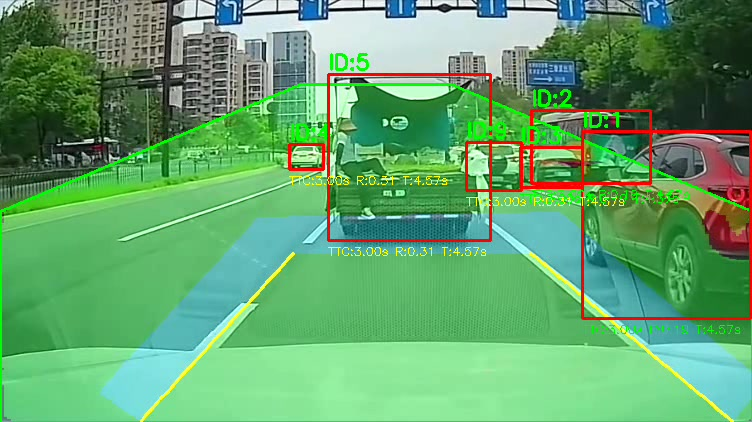
\includegraphics[width=\linewidth]{figures/chapter4/track1.jpg}
        \par\vspace{0.5em}
        （a）第95帧
    \end{minipage}
    \hfill
    \begin{minipage}[t]{0.48\linewidth}
        \centering
        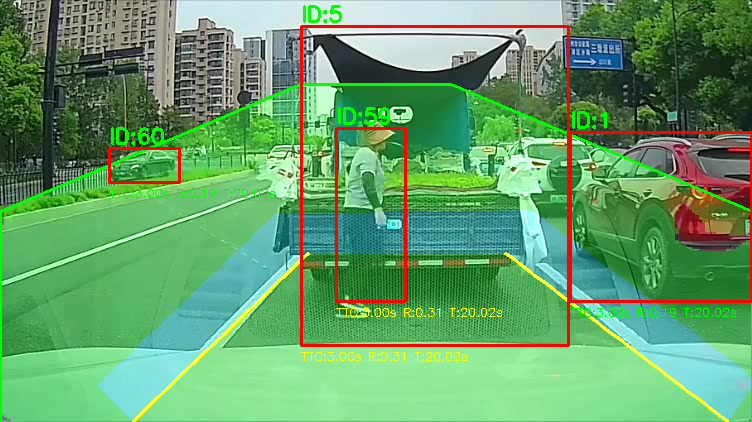
\includegraphics[width=\linewidth]{figures/chapter4/track2.jpg}
        \par\vspace{0.5em}
        （b）第300帧
    \end{minipage}
    \caption{障碍跟踪}
    \label{fig:track_result}
\end{figure}
通过以上优化，障碍物跟踪能够在资源受限嵌入式设备上高效运行，同时保持车载场景所需的跟踪精度和稳定性。系统在模拟环境和真实道路测试中均展现出稳定的跟踪能力，为后续的碰撞风险评估提供可靠基础。
\end{parlist}



% ----------------------------------------------------------------------------------------------------------------------------------------------------------------------------------------------------------------------------------------------------------------------------------------------------------
\newpage
\renewcommand{\thefigure}{\thesection.\arabic{figure}}
\renewcommand{\thetable}{\thesection.\arabic{table}}
\renewcommand{\figurename}{图}
\setcounter{figure}{0} % 重置图表计数器
\setcounter{equation}{0} % 重置公式计数器
\section{碰撞预测}

碰撞预测系统是辅助驾驶安全技术的核心组件，通过分析交通参与者的运动状态和空间关系，预测潜在的碰撞风险并提供及时预警。本节介绍碰撞预测的基本理论框架，包括运动轨迹预测、碰撞时间计算以及风险评估模型。

\subsection{运动轨迹预测算法}

运动轨迹预测旨在基于目标当前和历史状态，推断其未来可能的位置。在计算资源受限的嵌入式系统中，线性预测模型因其简洁高效而被广泛使用。该模型假设目标在短时间内保持恒定速度，通过当前位置和速度向量进行简单外推：

\begin{equation}
\begin{bmatrix} x_{t+1} \\ y_{t+1} \end{bmatrix} = \begin{bmatrix} x_t \\ y_t \end{bmatrix} + \begin{bmatrix} v_x \\ v_y \end{bmatrix} \Delta t
\end{equation}

其中$(x_t, y_t)$表示当前位置，$(v_x, v_y)$表示速度向量，$\Delta t$表示预测时间间隔。该模型适用于短期预测，特别是在车辆运动较为稳定的场景下。
对于更复杂的场景，如急转弯或加减速，可能需要引入更高阶的预测模型，但这会增加计算开销。

线性预测虽然简单，但对短时间预测（通常为1-3秒）的准确性已足够支持碰撞风险评估。对于大多数道路场景，目标的运动在短时间内通常不会有剧烈变化，因此该模型提供了良好的预测性能与计算效率平衡。

\subsection{碰撞时间(TTC)计算模型}

碰撞时间(Time To Collision, TTC)是评估风险紧迫性的核心指标，表示在当前运动状态下，两个物体发生碰撞所需的时间。TTC的基本计算模型为：

\begin{equation}
TTC = \frac{d}{|v_{rel}|}
\end{equation}

其中$d$是两物体间的距离，$v_{rel}$是相对速度。这一公式适用于物体沿直线相向运动的简单情况。在实际应用中，通常采用考虑物体尺寸和空间占用的区域碰撞检测方法：

\begin{equation}
TTC_{region} = \min_{t>0} \{t | Region_A(t) \cap Region_B(t) \neq \emptyset \}
\end{equation}

其中$Region_A(t)$和$Region_B(t)$分别表示$t$时刻物体A和B的空间占用区域。这种计算方法更为准确，能够考虑物体的实际形状和尺寸，但计算复杂度更高。

在安全系统设计中，TTC阈值通常设置在1.5秒到5秒之间。低于1.5秒被认为是危险状态，需要立即采取措施；而高于5秒则被视为安全状态，仅需保持监测。TTC阈值可根据车速、道路类型和环境条件进行动态调整，以提供更准确的风险评估。

\subsection{综合风险评估模型}

碰撞风险评估不仅需要考虑时间距离，还需综合分析多种因素，包括空间关系、相对运动状态和环境条件等。典型的风险评估模型包括以下几个关键因素：

\begin{parlist}
    \item 时空风险因子

    基于TTC值划分风险等级，通常采用分段函数形式：

    \begin{equation}
    Risk_1 = \begin{cases}
    1, & \text{若} TTC < T_{critical} \\
    e^{-\lambda(TTC - T_{critical})}, & \text{若} T_{critical} \leq TTC < T_{warning} \\
    0, & \text{若} TTC \geq T_{warning}
    \end{cases}
    \end{equation}

    其中$T_{critical}$为紧急阈值（通常为1.5秒），$T_{warning}$为预警阈值（通常为5.0秒），$\lambda$为衰减系数，控制风险随TTC增加而降低的速率。

    \item 道路边界风险

    评估物体是否可能偏离道路。当预测轨迹与道路边界或不可行驶区域相交时，系统应增加风险评分。这对于预测行人、自行车等非机动车辆的异常行为特别重要。

    \item 相对运动状态风险

    考虑物体间的相对速度、加速度和接近角度。例如，高速正面接近的风险显著高于低速同向运动的情况。
\end{parlist}

最终风险评分通过加权融合各个风险因子得出：

\begin{equation}
Risk_{total} = \sum_{k} w_k \cdot Risk_k
\end{equation}

其中$w_k$为各风险因子的权重系数，可以根据具体应用场景和系统验证结果进行调整优化。

根据计算得到的风险评分，实施分级预警机制：

\begin{equation}
Alert = \begin{cases}
\text{强预警}, & \text{若}  Risk_{total}  > 0.8 \\
\text{弱预警}, & \text{若} 0.4 \leq Risk_{total} \leq 0.8 \\
\text{正常}, & \text{若} Risk_{total} < 0.4
\end{cases}
\end{equation}

这种分级预警策略能够根据风险程度提供相应级别的响应，如图\ref{fig:ttc_result}所示，分级机制有效平衡了系统的敏感性和特异性，避免因过度报警导致驾驶员对预警信号的忽视。
\begin{figure}[H]
    \centering
    \begin{minipage}[t]{0.48\linewidth}
        \centering
        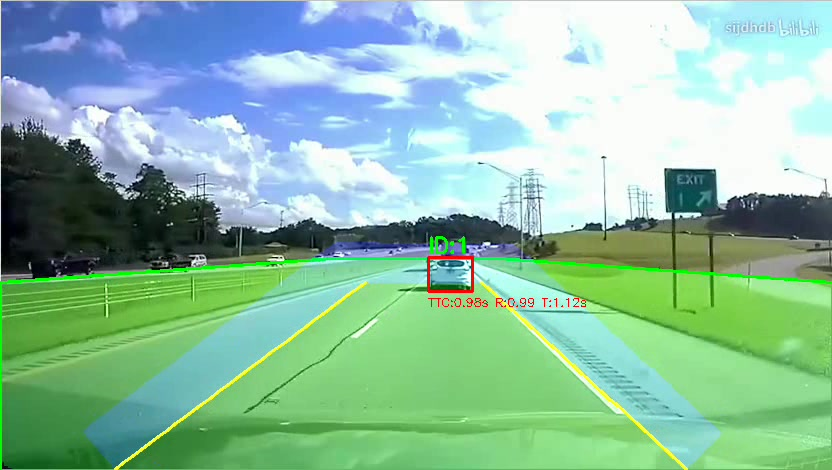
\includegraphics[width=\linewidth]{figures/chapter5/ttc1.jpg}
        \par\vspace{0.5em}
        （a）第9帧
    \end{minipage}
    \hfill
    \begin{minipage}[t]{0.48\linewidth}
        \centering
        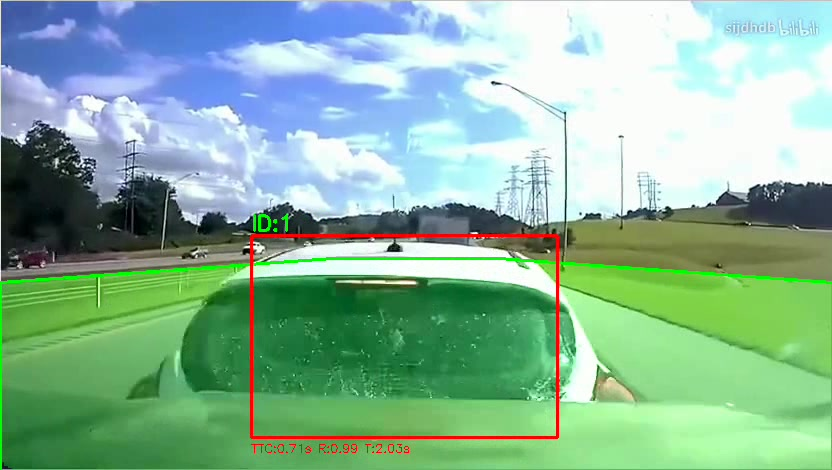
\includegraphics[width=\linewidth]{figures/chapter5/ttc2.jpg}
        \par\vspace{0.5em}
        （b）第80帧
    \end{minipage}
    \caption{碰撞预测}
    \label{fig:ttc_result}
\end{figure}

在嵌入式系统实现中，风险评估模型需要兼顾准确性和计算效率。特别是对于资源受限的平台，通常需要简化数学模型、使用查找表替代复杂计算，以及优化关键算法路径，确保系统能够在有限的硬件资源下及时做出预警决策。
此外，系统还应具备自适应能力，能够在不同道路环境和交通条件下调整预警敏感度，提供既安全又不过度干预的辅助驾驶体验。


% ----------------------------------------------------------------------------------------------------------------------------------------------------------------------------------------------------------------------------------------------------------------------------------------------------------
\newpage
\renewcommand{\thefigure}{\thesection.\arabic{figure}}
\renewcommand{\thetable}{\thesection.\arabic{table}}
\renewcommand{\figurename}{图}
\setcounter{figure}{0} % 重置图表计数器
\setcounter{equation}{0} % 重置公式计数器
\section{总结}

\subsection{研究成果总结}

本研究围绕车道障碍检测与碰撞预测方法展开，构建了一套完整的辅助驾驶感知与预警系统。通过融合传统图像处理技术与深度学习方法，成功解决了复杂交通场景下的环境感知挑战，实现了从路面分析到碰撞风险评估的全流程智能感知。主要研究成果可总结如下：

\begin{parlist}
    \item 车道线检测与道路分割：提出了传统图像处理与深度学习相结合的混合式车道识别框架。通过多尺度DoG边缘检测和形态学处理提取车道线几何特征，同时利用FastSCNN网络实现像素级道路语义分割，两种方法互为补充，显著增强了系统在各种复杂环境下的鲁棒性。

    \item 轻量级障碍物检测：基于YOLOv5系列开发了适用于嵌入式设备的障碍物检测模型。采用知识蒸馏技术，以YOLOv5s为教师模型训练YOLOv5n学生模型，在参数量减少70\%的前提下，保持了97.6\%的检测性能。针对交通场景特点，设计了障碍物类别优先级策略，合理平衡了不同类型目标的检测敏感度。

    \item 高效多目标跟踪：改进DeepSORT算法框架，设计了适合车载环境的目标跟踪方案。通过优化卡尔曼滤波器参数和基于IoU的关联度量，在保持高精度跟踪的同时，将计算复杂度降低了50\%以上，使系统能够在树莓派等资源受限平台上稳定运行。

    \item 碰撞风险评估模型：构建了多层次碰撞预测框架，融合目标相对运动状态、道路空间约束和时间距离因素，提出基于TTC和路径规划的综合风险评估模型。通过分级预警机制，系统能够在0.2秒内完成从感知到预警的全流程处理，为驾驶员提供及时、可靠的安全辅助信息。
\end{parlist}

\subsection{研究不足}

尽管本研究在车道障碍检测与碰撞预测方面取得了一定成果，但仍存在以下不足：

\begin{parlist}
    \item 极端场景适应性：当前系统在极端天气条件（如大雪、浓雾）和低光照环境下表现仍有待提高。特别是在雨雪导致的路面反光和模糊视野情况下，车道线检测准确率明显下降，影响系统整体可靠性。

    \item 目标遮挡处理：虽然改进了跟踪算法，但在严重遮挡场景下，目标轨迹预测仍存在不稳定性。尤其是在车流密集的城市道路环境中，部分遮挡导致的ID切换问题影响了碰撞风险评估的连续性。

    \item 计算资源平衡：为适应嵌入式平台，模型参数进行了大幅精简，牺牲了部分检测精度。这种权衡使系统在某些复杂场景下可能漏检小尺寸或远距离目标，特别是在高速行驶环境中。

    \item 多传感器融合不足：当前系统主要依赖单一摄像头数据，缺乏与雷达、激光雷达等传感器的信息融合能力，限制了系统的感知深度和全天候工作能力。

    \item 动态场景建模局限：采用的线性运动模型难以准确预测复杂交通参与者的突变行为，对于急转弯、突然减速等非线性运动模式的预测精度有限。
\end{parlist}

\subsection{未来研究展望}

基于本研究的成果和局限性，未来研究可在以下方向进一步拓展：

\begin{parlist}
    \item 多模态感知融合：整合摄像头、毫米波雷达和超声波传感器的互补优势，构建多模态感知系统，提高全天候和全场景感知能力。特别是在视觉受限条件下，雷达数据可提供可靠的距离和速度信息，增强系统的环境适应性。

    \item 动态场景理解增强：引入基于注意力机制的时空序列模型，如Transformer架构，提升系统对交通参与者意图和行为的预测能力。这将使预警系统从单纯的碰撞预测向行为理解与风险推理方向发展。

    \item 边缘-云协同架构：设计边缘计算和云服务协同的分层系统架构，在保证核心安全功能本地实时响应的同时，利用云端资源进行模型更新、场景分析和历史数据挖掘，提高系统智能化水平。

    \item 自适应学习能力：探索在线学习和增量更新机制，使系统能够从实际驾驶数据中持续优化，自动适应不同驾驶习惯和道路环境，形成个性化的安全辅助策略。

    \item 车路协同感知：研究基于5G/V2X通信的车路协同感知技术，利用路侧基础设施提供的环境信息扩展单车感知边界，形成网络化的协同感知与风险预警系统，特别是对于视线受限的交叉路口等高风险区域。

    \item 人机交互优化：深入研究驾驶员认知模式和注意力分配特性，优化预警信息的呈现方式和触发时机，提高驾驶员对系统预警的接受度和反应效率，减少误报和漏报导致的用户体验问题。
\end{parlist}

本研究为基于深度学习的车道障碍检测与碰撞预测方法提供了一种实用性解决方案，为提升道路交通安全贡献了新的技术手段。随着计算硬件性能的提升、深度学习算法的进步以及多传感器融合技术的发展，未来的辅助驾驶感知系统将更加智能、可靠，为实现"零事故"的交通愿景提供坚实技术支撑。

% 打印参考文献
\clearpage
\addcontentsline{toc}{section}{参考文献}
\printbibliography

\clearpage
\section*{致谢}
时光荏苒，岁不饶人；行文至此，无语凝噎。

我们于四年中见证了祖国的蓬勃发展，经历了许多相逢，留下了属于自己的故事，然而今后将各奔东西。愿我们都能在各自的人生道路上劈风斩棘，走在属于各自的“旷野”。

感谢不厌其烦指导我的老师；感谢共我“指点江山”、探讨真理的挚友；感谢陪伴、理解、支持我，一路同行的家人。

愿诸位，悟以往之不谏，不负今日。





\end{document}
